\documentclass[12pt,a4paper]{report}
\usepackage[utf8]{inputenc}
\usepackage[T1]{fontenc}
\usepackage{amsmath}
\usepackage{amsfonts}
\usepackage{amssymb}
\usepackage{graphicx}
\usepackage{ulem}
\usepackage{natbib}
\usepackage[a4paper,margin=1in,footskip=0.25in]{geometry}
\usepackage{float}
\usepackage{array,multirow,makecell}
\usepackage{indentfirst}
\usepackage[french]{babel}
\usepackage{graphicx, url}
\usepackage{float}
\usepackage{hyperref}
\usepackage{titling}
\usepackage{blindtext}
\usepackage{txfonts}
\usepackage{mathdots}
\usepackage[classicReIm]{kpfonts}
\setcellgapes{1pt}
\makegapedcells
\newcolumntype{R}[1]{>{\raggedleft\arraybackslash }b{#1}}
\newcolumntype{L}[1]{>{\raggedright\arraybackslash }b{#1}}
\newcolumntype{C}[1]{>{\centering\arraybackslash }b{#1}}


\begin{document}
	
	\begin{titlepage}
		\centering
		
\includegraphics[width=0.15\textwidth]{logo.jpg}\par
		\vspace{1cm}
		{\scshape\LARGE Universite Constantine 2 Abdelhamid Mehri \par}
		\vspace{1cm}
		{\scshape\Large Projet de fin d'études\par}
		\vspace{1.5cm}
		{\huge\bfseries Système de localisation en intérieur\par}
		\vspace{2cm}
		{\Large\itshape Seghiri Taki Eddine et Benchetra Hamza\par}
		\vfill
		Encadré by\par
		Dr. Belguidoum Meriem.
		
		\vfill
		{\large \today\par}
	\end{titlepage}
	
	\tableofcontents
	\listoffigures
	
	
\part{État de l'art.}

\chapter{Étude sur le positionnement en intérieur.}


\section{Introduction}

\smallskip
La localisation géographique d'objets, services ou personnes est devenue un besoin omniprésent  dans le quotidien. Evoluant à grande vitesse, les besoins sont toujours plus spécifiques ce qui implique que les techniques et technologies doivent elle aussi évoluer constamment pour satisfaire ces derniers.\smallskip

De nos jours, le GPS s’impose en \textit{outdoor}, offrant une précision métrique, cependant, dans les espaces clos, cette technologie peine a fournir des résultats fiable a cause des signaux affaiblit voir même bloqués par les obstacles les rendant inefficaces au regard des résultats souhaiter par les utilisateurs.

Ainsi, avec l’omniprésence d’infrastructures sans fil au sein des espaces clos, de nouvelles technologies de positionnement en intérieur peuvent être déployé pour prendre le relai des technologies existantes, notamment le GPS.

Certains systèmes opèrent dans des lieux publics tels que les musées ou parkings souterrains a des fins de guidage ou suivi de position en temps réel, d’autres dans le commerce, en prenant connaissances des déplacement habituels de l’utilisateur pour créer de l’interactivité en fonction du lieu où il se trouve.

Ces systèmes peuvent également être utilisés dans un but de surveillance. Les technologies de localisation peuvent permettre le suivi de personnes sensibles telles que des enfants ou des personnes âgées (par exemple).

De tels systèmes contribuent aussi au domaine de l’IoT. Les systèmes de positionnement en intérieur permettent de localiser toute entité munie d’un tag et les localiser les unes par rapport aux autres.


La localisation indoor soulève donc de nouveaux défis de conception et d’installation. Les systèmes de positionnement, désormais déployés en environnement dynamique, doivent allier robustesse et fiabilité tout en répondant à des exigences de précision, de temps critique, d’efficacité énergétique et de coûts de déploiement.

\section{Historique}

Dans le passé, pour déterminer sa localisation l'homme utilisait des méthodes primitives telles que le calcule d'angles entre l'horizon et le soleil à midi à l'aide d'outil particuliers, ainsi qu'une horloge pour déterminer la longitude, mais ces techniques n'étaient utilisables qu'à certains moments de la journée et dans des conditions météorologiques adéquates. Après cela, pendant les années 70 les forces militaires ont mis au point un système de localisation reposant sur un ensemble de 32 satellites chacun emmenant un signal unique et en continue a une vitesse constante ce qui fait que chaque signale arrive à une heure différente permettant ainsi de calculer la distance entre l'appareil et le satellite. Cette technique fut mise à la disposions au particuliers aux alentours des années 80 qui l'intégrèrent au téléphones portables et au véhicules. La détermination de la position se faisait ensuite à l'aide d'un algorithme de trilatération qui consiste à calculer la position à l'aide de trois distances pour un plan et de quatre pour une sphère (la terre). Avec le temps la localisation avec satellite à évoluer au point de fournir une précision à l'ordre de quelques mètres, ce pendant elle n'était efficace qu'en dehors des bâtiments et des espaces clos et c'est ici qu'interviennent les systèmes de localisation en intérieur qui remplace les systèmes de géolocalisation par satellite dans les milieux fermés.

\section{Définitions et terminologie }

\subsection{Géolocalisation par satellites}

La géolocalisation par satellite est un procédé de localisation qui consiste à émettre des signaux qui sont capté par un terminal qui calcule la latitude la longitude et parfois aussi l'altitude et au moins 4 satellites doit être visible du terminal, les exemples les plus connues sont le GPS le système de positionnement universelle américain Navstar NS-7B où ça variantes européenne nommé Galileo.

\subsection{RSSI (Received Signal Strength Indication)}

Une premièremétrique de radio-localisation, très souvent déjà mise à profit dans les systèmes de communication radio tel que les réseaux cellulaires etWLAN, s’appuie sur la mesure de la puissance du signal reçu, notée RSS (Received Signal Strength) pour décrire la puissance analogique reçue ou RSSI (Received Signal Strength Indicator) après quantification de cette même puissance par un récepteur réel.\cite{PHD:rssi}

\subsection{RTLS}

RTLS (Real-time locating systems) est une technologie de positionnement et d'identification qui a été prouvée dans divers marchés. Elle est utilisée pour identifier et suivre automatiquement des personnes ou des objets en temps réel, en général dans un bâtiment ou une zone limitée. Des tags RFID (Radio Frequency Identification) sans fil sont attachés à des objets ou portés par des personnes, et dans la plupart des applications RTLS les points de référence fixés reçoivent des signaux des tags RFID actifs ou passifs pour déterminer leur emplacement\cite{rtls}


\subsection{GPS: GLOBAL Positioning System}

Le Global Positioning System (GPS) (en français : « Système mondial de positionnement » [littéralement] ou « Géo positionnement par satellite »), originellement connu sous le nom de Navstar GPS, est un système de positionnement par satellites appartenant au gouvernement des États-Unis. Mis en place par le département de la Défense des États-Unis à des fins militaires à partir de 1973, le système avec 24 satellites est totalement opérationnel en 1995 et s'ouvre au civil en 2000\cite{gps}


\subsection{Ultra Wide Band (UWB)}

La transmission à ultra-large bande (UWB) est une technologie largement utilisée dans les applications de radar et de télédétection et a récemment reçu une grande attention dans les universités et l'industrie pour les applications de communications sans fil. Un système UWB est défini comme tout système radio dont la largeur de bande de 10 dB est supérieure à 25 pour cent de sa fréquence centrale, ou dont la largeur de bande de 10 dB est égale ou supérieure à 1,5 GHz si la fréquence centrale est supérieure à 6 GHz \cite{uwb}

\subsection{Bluetooth}

Bluetooth is a universal radio interface in the 2.45 GHz frequency band that enables portable electronic devices to connect and communicate wirelessly via short-range, ad hoc networks. Each unit can simultaneously communicate with up to seven other units per piconet. Moreover, each unit can simultaneously belong to several piconets \cite{bluetooth}

\subsection{Wifi}

le wi-fi ou la fidélité sans file en anglais est un ensemble de protocoles de communication qui fonctionne avec des ondes radio dans une bande passante entre [2.4 - 5 ] GHz , il est destiné au relie des équipement informatiques et de téléphonie mobiles dans un seul reseau haut débit et sans fil (WLAN)

\subsection{Wlan}
Un réseau sans fil (en anglais : wireless network) est un réseau informatique numérique qui connecte différents postes ou systèmes entre eux par ondes radio. Il peut être associé à un réseau de télécommunications pour réaliser des interconnexions à distance entre nœuds. (Réseau sans fil) \cite{wlan}


\subsection{Radio-identification}
	La radio-identification, le plus souvent désignée par le sigle RFID (de l’anglais radio frequency identification), est une méthode pour mémoriser et récupérer des données à distance en utilisant des marqueurs appelés « radio-étiquettes » (« RFID tag » ou « RFID transponder » en anglais). (Radio-identification)\cite{rfid}

\subsection{Trilatération}

La trilatération est une méthode mathématique permettant de déterminer la position relative d'un point en utilisant la géométrie des triangles tout comme la triangulation. Mais contrairement à cette dernière, qui utilise les angles et les distances pour positionner un point, la trilatération utilise les distances entre un minimum de deux points de référence.\cite{trilateration}


\section{Domaines d’application des systèmes de positionnement en intérieur}

\subsection{Aide à la navigation}
Dans le cas d’une navigation allant de l’outdoor à l’indoor (ex : Un client tilisant son application GPS pour se rendre de chez lui à un point d’intérêt précis situé à l’intérieur d’un centre commercial), celle-ci se doit d’être « sans coutures » : le mobile devra immédiatement détecter que l’utilisateur est rentré dans un bâtiment, et passer de manière transparente en mode navigation intérieure.
Sites industriels Une fois un problème identifié sur un site industriel, une application mobile pourrait permettre de guider l’équipe technique mobile la plus proche vers la source du problème. Ensuite, une fonctionnalité d’aide à la résolution de problème type Réalité augmentée ou Télé-assistance pourrait prendre le relai si besoin\cite{navigation}


\subsection{Transport}
Permettre à un voyageur de naviguer non seulement en extérieur, mais aussi à l’intérieur d’un lieu de type aéroport, gare ou station de métro\cite{transport}% ya tzid ya tne7iha

\subsection{Supermarchés et Hypermarchés}
Supermarchés et Hypermarchés
Les grandes surfaces comme les supermarchés nécessitent des compétences de localisation pour se situer dans les rayons et de trouver les articles recherchés, un système de localisation dans un tel endroit permettra de montrer aux clients les emplacements des produits ou rayons et faciliter leur expérience d’utilisateur.
Le système peut même être utilisé pour des buts publicitaires comme par exemple faire des propositions aux clients selon leurs préférences ou de liquider des produits etc.


\subsection{Marketing}

la principale application du marketing serait le géomarketing : l’optimisation des revenus au mètre carré, en fonction des données de visite des clients (flux, temps de visite, zones de passages, zones de transformation, etc.). Il est possible de personnaliser des offres marketing, non seulement selon les données connues sur le client par la marque (carte de fidélité) mais aussi selon le contexte géographique d’un client en magasin.


\section{Technologies utilisées}

Les technologies mettant à l’œuvre des systèmes de localisation indoor se distinguent en deux catégories :


– Des technologies autonomes ne nécessitant aucune infrastructure à déployer, donc sans interaction entre l’utilisateur et des équipements.


– D’un autre côté, celles reposant sur une infrastructure d’équipements interconnectés.

\subsection{Les technologies autonomes}

\textbf{-Capteurs inertiels et dead reckoning :}


	Ces premiers systèmes de positionnement s’appuient sur une méthode appelée de « dead reckoning »\cite{dead} , qui consiste à déduire la position actuelle à partir de la position précédente.
	
	Le système exploite donc les capteurs inertiels (accéléromètres, gyroscopes, etc.) parfois utilisés en combinaison avec la boussole ou le podomètre intégré de l’appareil mobile. Ces différents dispositifs permettent de calculer les déplacements dans l’environnement. L’utilisateur doit disposer d’un smartphone ou d’une carte embarquée contenant des capteurs inertiels et le plan du bâtiment doit être connue, aussi, il est nécessaire de connaitre l’emplacement initial de l’utilisateur.
	
	Les données de déplacement recueilli pendant le mouvement du porteur du dispositif permet de déterminer la nouvelle position qui calculé de manière relative, la position à l’instant T-1 permettant de déterminer celle à l’instant T. Une communication entre la carte ou l’appareil mobile peut entrer en jeux a fin de centraliser les données et réduire la charge de calcule sur le terminal
	
	
\textbf{	Atouts et faiblesse :}
	
	Ces systèmes ont l’avantage d’être pratiquement autonomes en présences des conditions adéquates. Mais leur précision de positionnement reste toutefois limitée à causes des erreurs cumulées au fil des déplacements.
	
	
	Les  capteurs inertiels sont généralement utilisés en combinaison avec d’autres technologies, selon le principe de fusion des données.
	
	\begin{itemize}
	\item Étude des champs magnétiques \cite{magnet}
	
	Cette technique se base sur des capteurs a effet Hall afin de mesurer l’intensité des champs magnétiques terrestres présents au sein des espaces clos, champs magnétiques dont l’intensité diffère d’un emplacement à un autres à causes des perturbations causées par les structures métalliques composants le bâtiment. En enregistrant les variations de ces derniers, une détermination de la position est possible
	
	
	Bien qu’elle soit indépendante de toute interaction avec des périphériques externes, cette technique de localisation nécessite toutefois une calibration initiale en plus de l’acquisition d’informations spécifiques à l’environnement de déplacement
	
	Deux approches sont donc possibles :
	
	
	– pour chaque position du champs , l'utilisation de ses valeurs mesurées sur différents axes
	
	– La reconnaissance de patterns représentatifs d’un élément
	
	La première démarche s’appuie sur le principe de « Fingerprinting ». Qui consiste a enregistrer les différentes intensités du champ magnétique sur les axes de déplacements (x, y, z) dans différents points de l’environnement, qui soit dit en passant doit être cartographier au préalable, grâce au capteur a effet Hall et sauvegarder les valeurs recueilli dans une base de données.
	
	\begin{figure}[h]
		\centering
		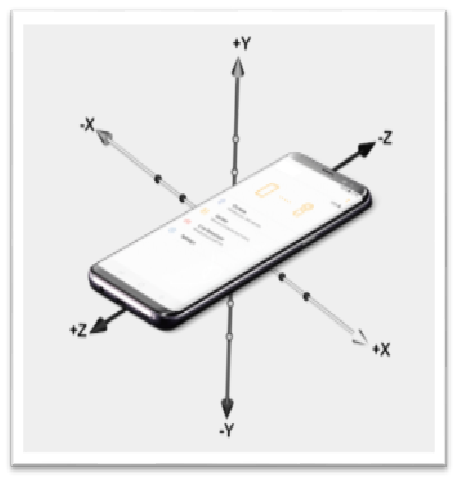
\includegraphics[width=0.4\linewidth]{Pics/position.png}
		\caption{Repère d’étude lié à l’appareil embarqué.}
		\label{fig:position}
	\end{figure}

ensuite, a la phase de déplacement libre , le dispositif (téléphone par exemple) compare les valeurs actuelles avec les valeurs qui se trouve dans la base de données précédemment constituée. Il repère alors l’usager à la position correspondante.


 \textbf{Atouts et faiblesses :}


Bien que cette technique ne soit pas très populaire, la localisation via champ magnétique prometteuse et pas très couteuse. Elle offre une précision jusqu’à maintenant inférieure à un mètre, et tout ça, sans l’exigence d’une infrastructure. 

Toutefois l’utilisation d’une telle technologie se limite à des situations bien spécifiques. En effet, pour pouvoir l’utiliser, les déplacements de l’utilisateur doivent être prévisibles et former un pattern plus ou moins précis par exemple un supermarché avec des rayons ou un local avec des couloirs etroits.

De fait, la mobilité d'usager doit étre limitée , sous soucis d’avoir une complexité élevée
	


\subsection{Les technologies basées sur une infrastructure}

\item Les techniques d’imagerie

	Cette méthode consiste a équiper l’environnement de capteurs visuels comme des caméras,  dans des positions fixes et connues et qui identifieront les objets à localiser, elle repose sur le concept d’analyse environnementale afin d’extraire les anomalies. 

\textbf{Atouts et faiblesses :}

Les systèmes d’imagerie atteignent souvent une très bonne précision en espace clos, de plus ils ne nécessitent aucun dispositif rattaché à l’utilisateur, ce qui constitue un avantage certain (le système est dit « device free »).

Toute fois elles sont limitées en ce qui concerne le champ de vision, et en présences d’un nombre importants d’individus, il devient plus difficile de les identifier, bien sur  des solutions existent, mais cela requiert des capacités de calculs élevées, venant augmenter les coûts.

\item L’exploitation des ondes radio 

Avec leurs caractéristiques impressionnantes, les ondes radiofréquences peuvent traverser des cloisons, murs ou tout autre obstacle pouvant être présent au sein d’un bâtiment ou n’importe quel espace clôt. En plus, leur omniprésence au quotidien fait d’eux la base de nombreuses technologies de positionnement.

Plusieurs standards, et que l’on va citer dans ce qui suit, existent et chacun s’adapte a de nombreux cas d’utilisations. En général, l’architecture utilisée consiste en un ensemble de tag attachés aux personnes ou aux objets à localiser et d’un ensemble d’antennes déployer dans l’espace clos.

	\begin{figure}[H]
	\centering
	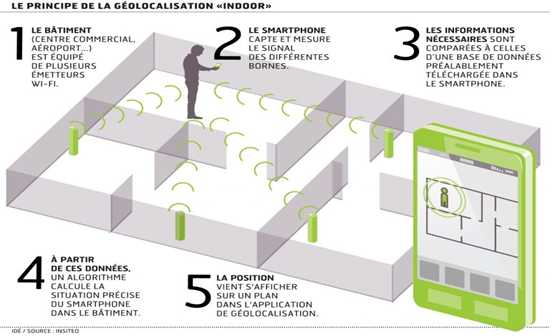
\includegraphics[width=0.8\linewidth]{Pics/indoor.png}
	\caption{Exemple d’utilisation des signaux Wi-Fi à des fins de localisation.}
	\label{fig:indoor}
\end{figure}
	Deux cas d'architecture sont alors possible:
	-Soit le dispositif (tag) émet et les capteurs (antennes) sont à l’écoute
	
	-Soit chaque capteur (antenne) émet à destination du dispositif (tag), qui se charge de traiter l’information
	
		\begin{figure}[H]
		\centering
		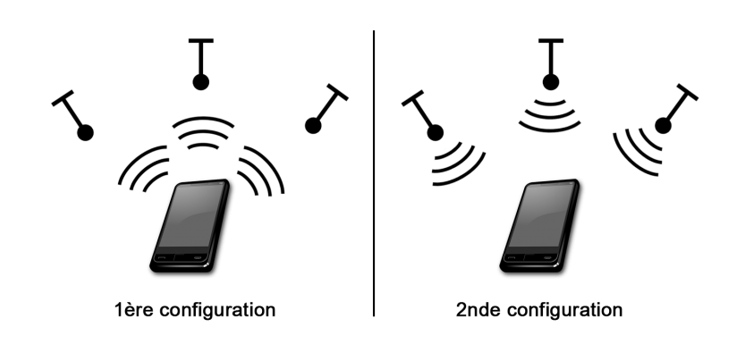
\includegraphics[width=0.8\linewidth]{Pics/architecture.PNG}
		\caption{Configurations possibles dans les systèmes de localisation en intérieur.}
		\label{fig:architecture}
	
\end{figure}

-Chacune de ces configurations offre plusieurs avantages :

\item La première permet de réduire les éléments actifs au sein du système. 

En effet, il n'ya que le dispositif (tag) qui est chargé d’émettre les signaux  vers les antennes environnantes, ce qui facilite énormément la synchronisation. Après réception du signal les antennes communiquent avec le serveur chargé du traitement algorithmique.


Grâce à cette approche, les ressources chargé du calcul nécessaires au niveau du dispositif (tag) sont minimiser, la position de l’usager est par contre rendue accessible pour tout les utilisateurs du serveur.

\item La deuxième configuration concentre tout le traitement au niveau de l’équipement à localiser, cela permet une position a temps réelsans avoir à un accès secondaire.
donc l'utilisation d'une connexion réseau n'est plus utile.


En pratique le choix de la solution est à la charge du concepteur, selon l’utilisation souhaitée et la technologie support. En somme, la figure suivante synthétise la classification du chapitre :

	\begin{figure}[H]
	\centering
	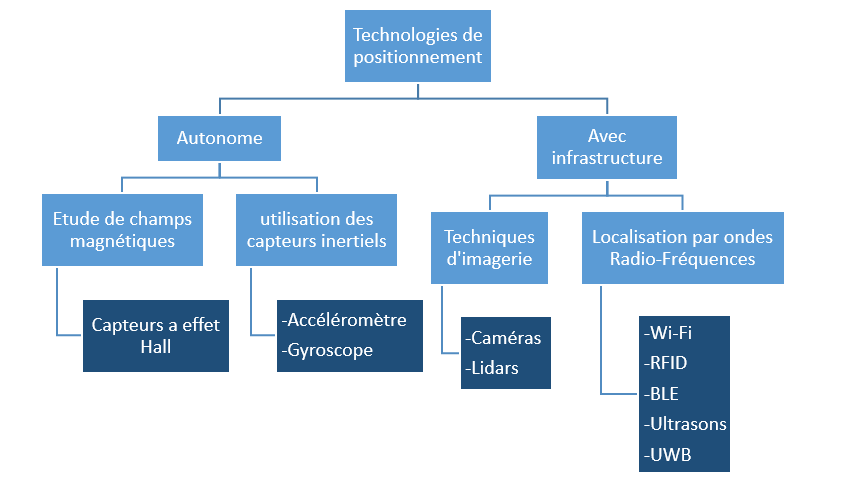
\includegraphics[width=1\linewidth]{Pics/techniques.PNG}
	\caption{Classification des technologies de positionnement indoor selon l’architecture à déployer.}
	\label{fig:techniques}
	
\end{figure}

La majorité des systèmes de localisation en intérieur utilisent des ondes radio comme moyen de communication. La transmission se fait entre un dispositif (tag) mobile et un réseau d’antennes fixés dans les angles d’endroit étudié.

selon la nature de l’information utile , les algorithmes de positionnement se subdivisent en plusieurs catégories , chacun d'eux s'adapte à : "la technologie supportée et l'espace ciblé".


\subsection{Synthèse des technologies}

Les forces et faiblesses des technologies précédentes peuvent être synthétisées à travers les tableaux suivants, le premier pour\textbf{ les technologies autonomes} et le second pour \textbf{les technologies basées sur les ondes}. 

Les paramètres de exactitude et de portée sont en comparaison. Ces indices sont dépendants de la densité de l’espace étudié, la nature des matériaux, …)

	\begin{figure}[H]
	\centering
	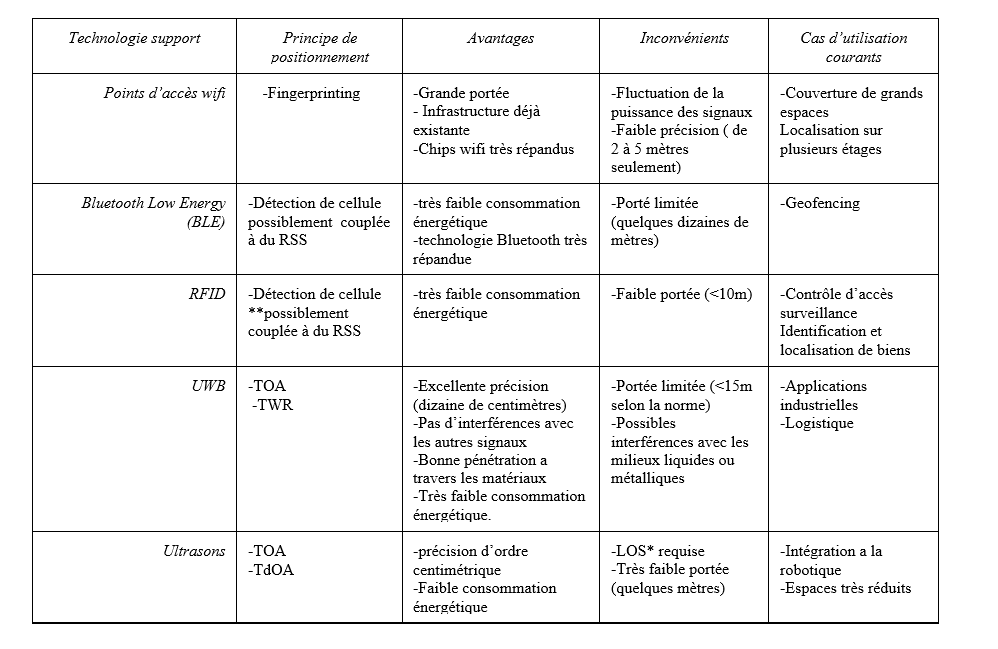
\includegraphics[width=1.1\linewidth]{Pics/technologies.PNG}
	\caption{Synthèse des technologies par ondes radios.}
	\label{fig:technologies}
	
\end{figure}



\section{Localisation en intérieur par ondes }

Localisation en intérieur par ondes 
Etant donné notre intérêt a la géolocalisation indoor par ondes radio nous présenterons ses divers principes et technologies. 

Une comparaison des différentes technologies ensuite est effectuée, permettant ainsi de préciser leurs différences en terme de caractéristiques et les cas d’utilisation courants.
Dans cette architecture les systèmes seront composée d’un dispositif mobile (tag) à localiser, ainsi qu'un réseau d’antennes, déployées au sein de l’espace étudié à des positions connues et préalablement enregistrées dans la base de données

\subsection{Techniques utilisées}
ndirou intro
\subsubsection{Méthode de mesure des angles d’arrivée (AOA)}

Cette méthode nommé "l’angle d’arrivée (Angle Of Arrival)" utilise les angles des signaux émis par le dispositif mobile vers deux antennes environnantes au minimum
Après détermination de ces angles, la position du dispositif est obtenue en intersectant les droites passantes par chaque point de reférence ce qui est appelé \textbf{la triangulation}

\begin{figure}[H]
	\centering
	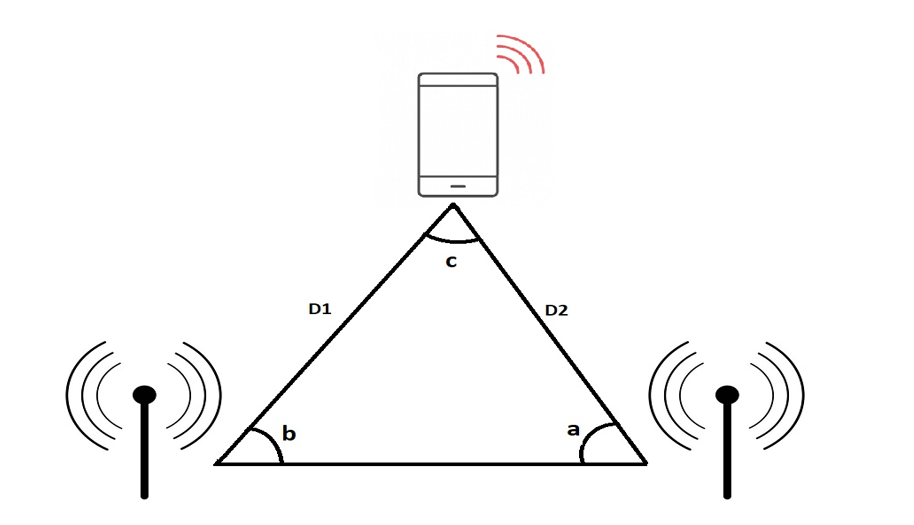
\includegraphics[width=0.5\linewidth]{Pics/triangulation.PNG}
	\caption{Principe de triangulation à partir de deux antennes réceptrices.}
	\label{fig:triangulation}
	
\end{figure}


Le principal avantage du ce processus est qu’il ne nécessite que deux antennes de référence pour qu'il détermine une position en espace 2D. Mais reste incapable lorsqu'il s'agit d'un dispositif émetteur qui se trouve dans la même ligne qu'un récepteur 


\subsubsection{Méthode de mesure des temps d’arrivée (TOA)}

Cette technique se base sur le temps de propagation d’un signal, entre l’émission par le dispositif (tag) mobile au moment Ti et la réception au sein du capteur (antenne) au moment Tf. Ces deux instants justifient la nomination de la technique, appelée  "Time Of Arrival".

ce temps de propagation est lié à une distance d tel que \textbf{d = c * (Tf – Ti)},

 Pour chaque capteur , une position est préalablement connue, l’usager se repère alors quelque part sur le cercle de rayon "d" et le point du centre "c" ou est situé le capteur (antenne) en question.
 
 cette opération est faite pour trois antennes au minimum , ce qui permet d’obtenir une position en espace bi-dimensionnelle (à l’intersection des 3 cercles construites). c'est la  « \textbf{trilatération} ».

\begin{figure}[H]
	\centering
	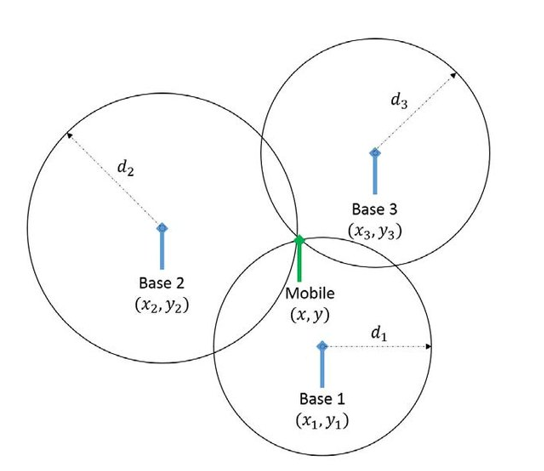
\includegraphics[width=1.1\linewidth]{Pics/trilateration.PNG}
	\caption{Principe de trilatération utilisé dans la méthode de TOA}
	\label{fig:trilateration}
	

\end{figure}

l'inconvénient majeur de cette technique est que la synchronisation entre les nœuds doit être extrêmement précise , Ainsi que l'horodatage exact doit être transmis a tout les antennes du réseau une fois un dispositif (tag) émet une trame.
\subsubsection{Méthode de mesure des différences de temps d’arrivée (TdOA)}

Son fonctionnement se résume en ces étapes : 

-un capteur (antenne) maître est en charge de partager son horloge aux autres récepteurs qui se trouve a son voisinage

 -Ensuite le dispositif (tag) émet régulièrement de courts messages diffusés en broadcast.
 
  La différence entre les temps d’arrivée du signal au paire de capteurs introduit une différence de distance entre l’usager et cet même paire.
  
  \textit{ Celui-ci se situe alors sur une hyperbole ayant pour foyer les deux récepteurs. Sa position exacte est finalement obtenue après réitération du processus, à l’intersection des hyperboles construites comme la figure ci dessous l'indique}
  
  

\begin{figure}[H]
	\centering
	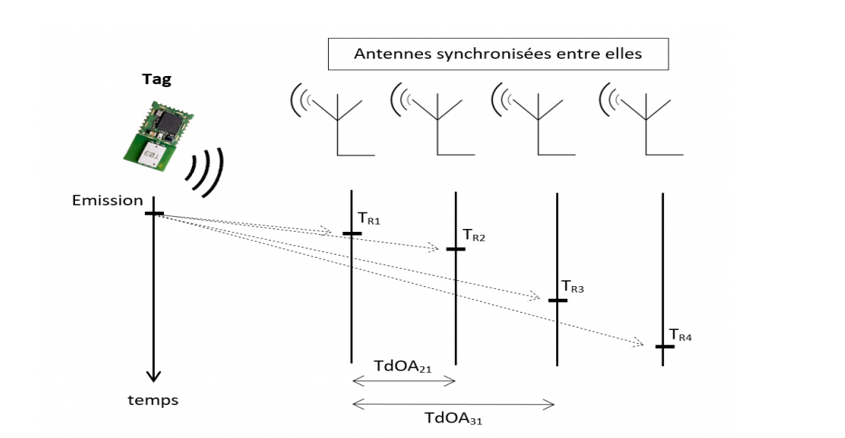
\includegraphics[width=1.1\linewidth]{Pics/tdoa.PNG}
	\caption{Illustration de la méthode de TDoA}
	\label{fig:tdoa}
	
	
\end{figure}

\subsubsection{Méthodes basées sur la puissance des signaux reçus (RSS)}

ces méthodes se basent sur la puissance du signal reçu (soit au niveau du dispositif cible (tag) soit au niveau des nœuds de référence (antennes fixes), selon le type d'émetteur. les algorithmes qui se basent sur la RSS (Received Signal Strength) se subdivisent en deux catégories.

\item ceux qui se basent sur une correspondance directe\textbf{ Puissance = fonction(distance)}. La puissance mesurée, au niveau du dispositif (tag) par exemple, est dite \textit{représentative de la distance} des antennes de référence, leur position est a présent connue.

une fois ces distances sont tenues en compte pour un minimum de trois antennes, le système utilise le principe de \textbf{trilatération} afin de marquer la position exacte du dispositif mobile. il existe plusieurs équations mathématiques qui permet de modéliser le comportement du canal, en quantifiant la puissance du signal en fonction de la distance parcourue. L’évolution est souvent logarithmique.


\begin{figure}[H]
	\centering
	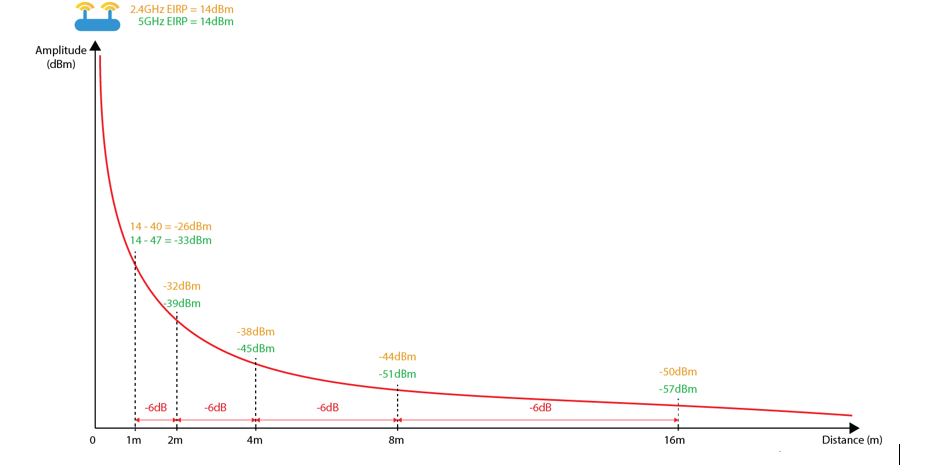
\includegraphics[width=1.1\linewidth]{Pics/rss.PNG}
	\caption{Exemple de l’évolution de la force du signal avec la distance (Technologie RFID)}
	\label{fig:rssi}
	
	
\end{figure}

\item
cette catégorie nécessite la création d’un jeu de donnée lors d’initialisation,nommé le \textbf{« Fingerprinting »}. la base de données est constituée en amont de la localisation.

 la base de données contient tous les relevés de puissance pour des positions fixes dans l'environnement étudié. 
 
 en supposant que les puissances de N tag émetteur peuvent etre observées à la position (x,y), ces informations sont sauvegardées et forment une empreinte 'Fingerprint':
 
 \begin{figure}[H]
 	\centering
 	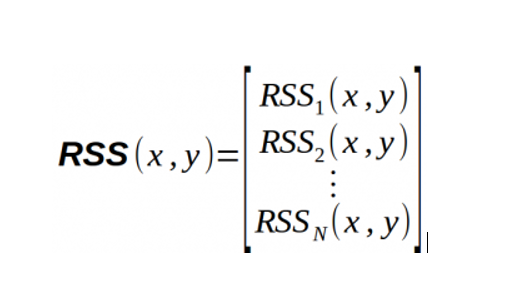
\includegraphics[width=0.5\linewidth]{Pics/sysRss.PNG}

 	
 	
 \end{figure}

Ce processus se répète régulièrement ce qui permet d’établir une  cartographie de l'environnement.
 \begin{figure}[H]
 	\centering
 	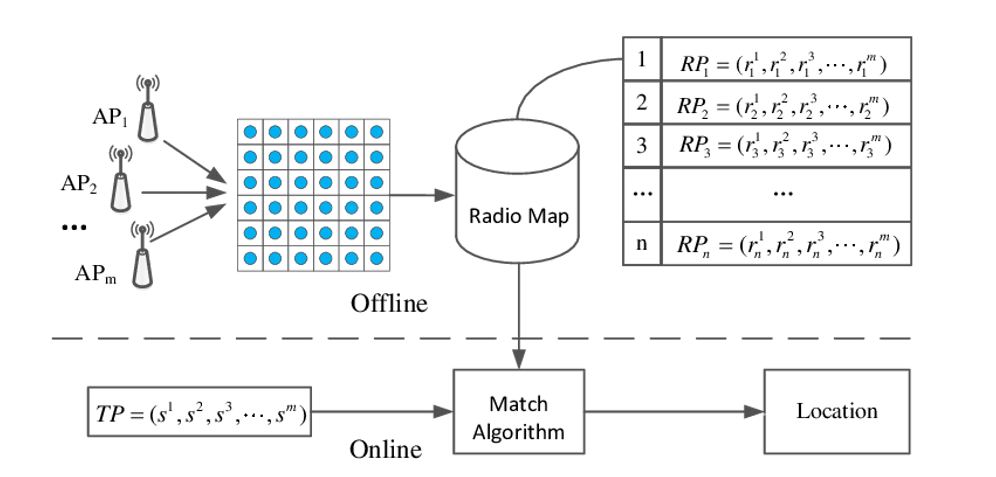
\includegraphics[width=1.1\linewidth]{Pics/sysRss2.PNG}
 	\caption{Illustration du principe de Fingerprinting}
 	\label{fig:sysRss2}
 	
 	
 \end{figure}

Lors du passage suivant a la période de localisation, l’appareil interroge la base de donnée pour affecter l’empreinte observée à une position dans l’environnement . 
La précision du positionnement est en relation directe avec le nombre de positions enregistrées et le nombre d'antennes déployées.





\paragraph{}
Cette seconde méthode de cartographie a pour mérite de tenir compte des spécificités du milieu. Les puissances observées reflètent les atténuations des murs ou du mobilier. La construction préalable de la base de données permet alors de répertorier les singularités de chaque position.	Ainsi le processus offre usuellement de meilleurs résultats en milieu dense, ce qui justifie son importante utilisation. A l’inverse, une simple corrélation distance/puissance est plus susceptible d’engendrer de lourdes imprécisions.



\subsubsection{Comparatif des techniques}

Les méthodes précédemment décrites admettent des atouts et faiblesses justifiant leur emploi selon le contexte. Ces caractéristiques sont résumées dans le tableau suivant :

  \begin{figure}[H]
 	\centering
 	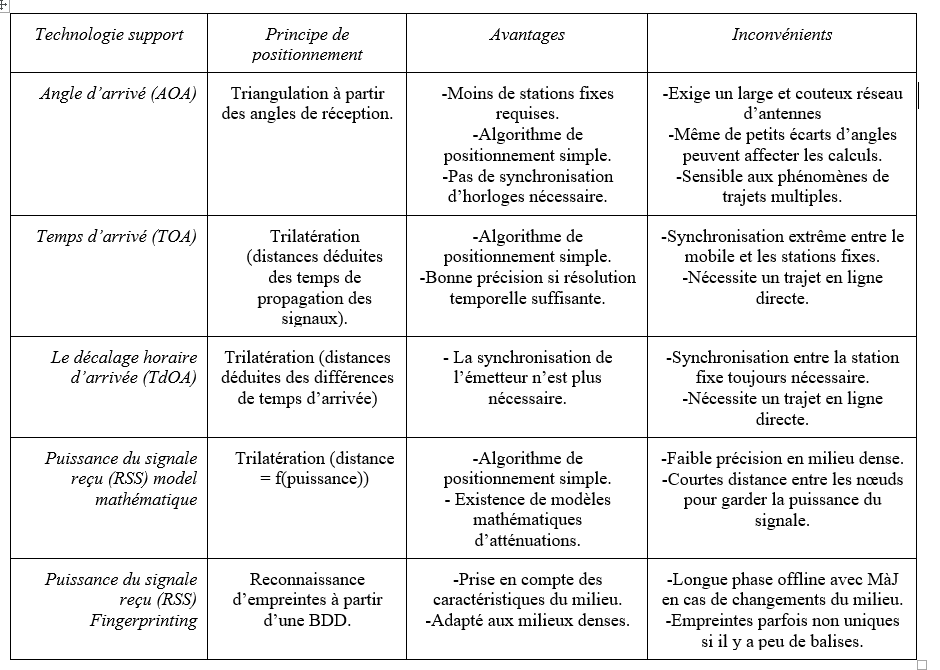
\includegraphics[width=1.1\linewidth]{Pics/tableau.PNG}
 
 	
 	
 \end{figure}
\end{itemize}

\section{Etude de l’existant }
\subsection{L’entreprise française Polestar}
Cette entreprise offre des services de localisation en intérieur en utilisant les réseaux sans fil disponibles à l’intérieur des bâtiments tel que le wifi ou le Bluetooth, elle combine aussi l’envoi d’information ciblées avec ses systèmes.

\subsection{L’entreprise anglaise Pointr Labs}
Cette entreprise utilise une approche de deep learning pour raffiner ses systèmes de localisation en intérieur, elle utilise aussi la technologie Li-Fi qui concise a transférer les données via la lumière, une technologie précise mais gourmande en terme de calcule et d’argent.

\subsection{L’aéroport de Londres-Gatwick }
« En 2017, L’aéroport Gatwick près de Londres en Angleterre a installé un système de « GPS intérieur » pour permettre aux voyageurs de trouver leur chemin dans ses terminaux grâce à leur téléphone multifonction. Environ 2000 balises communiquant en Bluetooth ont été installées au début de l’année sur une période de trois mois permettent ainsi d’indiquer une position géographique, à plus au moins trois mètres près. En comparaison, les points d’accès Wi-Fi, qui pourraient servir à localiser un téléphone, offrent une précision moindre, d’entre cinq et quinze mètres.\cite{WEBSITE:2}

\subsection{Hypermarché Carrefour  Westfield Euralille Lille, France}
Pour guider les consommateurs dans l'hypermarché, Carrefour Euralille a installé un système de géolocalisation en intérieur basé sur la lumière LED développé par Philips.
Pour mettre en œuvre ce system, il a fallu équiper le magasin de 7 800 M² de 2,5 km de rails de LED. Il y a près de 800 luminaires dans le magasin, chacun d'entre eux envoie à travers la lumière un code détectable par la caméra du smartphone. C'est comme du morse ou du binaire qui communique avec des 0 et des 1.\cite{WEBSITE:3}

\section{Conclusion}

Les travaux cités précédemment sont des exemples de travaux liés au sujet de notre mémoire chacun d’entre eux utilise une technologie différente et adaptée à son contexte. 
Dans notre cas, nous allons mettre en place un système standard pouvant être utilisé dans n’importe quel infrastructure du moment où l’en a accès à la cartographie de cette dernière.
Nous allons maitre au point un système de localisation qui combine à la fois technologie autonome et la technologie basées sur les ondes wifi, et ce, pour améliorer au maximum la précision de notre système et l’algorithme de trilatération vu que c’est l’algorithme le plus utilisé dans le domaine de localisation que ce soit en interne ou en externe et aussi a cause de sa simplicité et efficacité.


\chapter{Méthodologie.}

\section{Introduction}
Dans ce chapitre nous parlerons des outils et matériel utilisé dans la mise au point d'un système de localisation en intérieur en général puis ont terminera avec une comparaison

\noindent \begin{flushleft}
	
	
	\noindent 
	
	\noindent 
	
	\noindent 
	
	\noindent 
	
	\noindent 
	

	
	\noindent 
	
	\noindent 
	
	\noindent 
\end{flushleft}


\section{ Introduction}


	\paragraph
	D'abord pour entamer un projet on doit établir un plan de travail ainsi que sa conception , dans le monde informatique , les processus de travail definit plusieurs langages de conceptions , d'ou on a choisi le processus UP comme processus de développement qui sera définit par le langage SysML.
	\noindent Les méthodes de l'Ing\'{e}nierie Syst\`{e}me (IS) reposent sur des approches de mod\'{e}lisation et de simulation pour valider les exigences, et pour v\'{e}rifier ou \'{e}valuer le syst\`{e}me. La mod\'{e}lisation a donc couramment \'{e}t\'{e} utilis\'{e}e pour l'IS, que ce soit pour des repr\'{e}sentations concr\`{e}tes avec des plans ou
	
	\noindent mod\`{e}les r\'{e}duits, ou plus abstraites avec des syst\`{e}mes d'\'{e}quations.
	
	\noindent En g\'{e}n\'{e}ral l'IS tend \`{a} mod\'{e}liser les aspects suivants du syst\`{e}me: d\'{e}composition fonctionnelle, flux de donn\'{e}es, et d\'{e}composition structurelle. Exemples de techniques de mod\'{e}lisation employ\'{e}es :
	
	\noindent Le diagramme de flux de donn\'{e}es (DFD ou Data Flow Diagram) pour d\'{e}finir les donn\'{e}es traversant un syst\`{e}me et leurs traitements \'{e}ventuels
	
	\noindent Le diagramme de flux fonctionnel de bloc (FFBD ou Functional Flow Block Diagram) proche du diagramme UML d'activit\'{e} ou du "flowchart". 
	
	\noindent  La mod\'{e}lisation avec le langage UML est une pratique bien \'{e}tablie dans l'industrie logicielle. Bien que le langage UML permette par son caract\`{e}re \`{a} usage g\'{e}n\'{e}ral d'adresser de nombreux besoins pour l'IS, il est n\'{e}cessaire d'adapter ce langage de mod\'{e}lisation par la d\'{e}finition de  "profils UML".
	
	\noindent Le besoin de d\'{e}finir un langage bas\'{e} sur UML pour l'IS a \'{e}t\'{e} initi\'{e} en 2001 par l'organisation internationale de l'ing\'{e}nierie syst\`{e}me INCOSE (International Council on Systems Engineering).
	
	\noindent SysML (Systems ModelingLanguage) est bas\'{e} sur UML et remplace la mod\'{e}lisation de classes et d'objets par la mod\'{e}lisation de blocs pour un vocabulaire plus adapt\'{e} \`{a} l'Ing\'{e}nierie Syst\`{e}me. Un bloc englobe tout concept logiciel, mat\'{e}riel, donn\'{e}es, processus, et m\^{e}me la gestion des personnes.
	
	\noindent Comme repr\'{e}sent\'{e} sur le diagramme suivant, SysML r\'{e}utilise une partie d'UML, et apporte \'{e}galement ses propres d\'{e}finitions (extensions SysML) : 4 structurels, 4 dynamiques, et le diagramme d' exigences.
	
	\noindent Structurels :


\begin{enumerate}
	\item  Le " Block Definition Diagram " (BDD) remplace le diagramme de classes
	
	\item  L' "Internal Block Diagram" (IBD) remplace le diagramme de structure composite
	
	\item  Le diagramme de paquetage reste inchang\'{e}
	
	\item  Le diagramme param\'{e}trique est une extension SysML pour l'analyse de param\`{e}tres critiques
	
	\item  du syst\`{e}me.
\end{enumerate}

\noindent \begin{flushleft}
	Dynamiques :
\end{flushleft}

\begin{enumerate}
	\item  Le diagramme d'activit\'{e}s est l\'{e}g\`{e}rement modifi\'{e} pour SysML
	
	\item  Les diagrammes de s\'{e}quence, d'\'{e}tats, et de cas d'utilisations restent inchang\'{e}s
	
	\item  Le diagramme d'exigences est une extension SysML
\end{enumerate}

\noindent \begin{flushleft}
	
	
	\noindent 
	
	\noindent Ainsi SysML permet de fournir un r\'{e}f\'{e}rentiel central qui supporte les analyses du syst\`{e}me requises
	
	\noindent par l'IS, \`{a} savoir la d\'{e}composition fonctionnelle, les flux de donn\'{e}es, et la d\'{e}composition structurelle. 
	
	\noindent Chaque diagramme est nomm\'{e} d'une fa\c{c}on bien pr\'{e}cise et constitue un \'{e}l\'{e}ment nomm\'{e} du mod\`{e}le. 
	
	\noindent Pour cela SysML d\'{e}finit une en-t\^{e}te standard \`{a} chaque diagramme qui contient obligatoirement : 
	
	\noindent 
	
	\noindent De plus, chaque diagramme dispose d'une description :
\end{flushleft}

\begin{enumerate}
	\item  Version.
	
	\item  Description.
	
	\item  Statut ou niveau d'avancement.
	
	\item  R\'{e}f\'{e}rence, etc...
\end{enumerate}

\noindent \begin{flushleft}
	
\end{flushleft}


\section{ Diagrammes de SysML}

\noindent \begin{flushleft}
	
	
	\noindent Le langage sysML propose 9 types de diagrammes destin\'{e}s \`{a} repr\'{e}senter les aspects fonctionnel, structurel et comportemental d'un syst\`{e}me. 
	
	\noindent Pour mod\'{e}liser l'aspect fonctionnel :
\end{flushleft}

\begin{enumerate}
	\item  Le diagramme des cas d'utilisation (UCD) 
	
	\item  Le diagramme des exigences (RD)
\end{enumerate}

\noindent \begin{flushleft}
	
	
	\noindent Pour repr\'{e}senter l'aspect structurel :
\end{flushleft}

\begin{enumerate}
	\item  Du diagramme de d\'{e}finition de blocks (BDD) 
	
	\item  Du diagramme de block interne (IBD)
\end{enumerate}

\noindent \begin{flushleft}
	Pour mod\'{e}liser l'aspect comportemental :
\end{flushleft}

\begin{enumerate}
	\item  Le diagramme de s\'{e}quence (SD) 
	
	\item  Le diagramme d'\'{e}tat (STM)
\end{enumerate}


\subsection{ Description fonctionnelle}

\noindent \begin{flushleft}
	Trois diagrammes interviennent dans la mod\'{e}lisation fonctionnelle d'un syst\`{e}me.
	
	\noindent 
\end{flushleft}


\subsubsection{ Le diagramme des cas d'utilisation (UCD) :}

\begin{flushleft}
	
	
	\noindent Tout comme avec UML, on utilise les diagrammes de cas d'utilisations :
	
	\noindent 
\end{flushleft}

\begin{enumerate}
	\item  Bas\'{e} sur les interactions acteurs/syst\`{e}me, pour identifier les acteurs et les cas d'utilisations d'un point de vue utilisation du syst\`{e}me
	
	\item  Pour choisir et identifier les fronti\`{e}res, le p\'{e}rim\`{e}tre fonctionnel du syst\`{e}me
\end{enumerate}

\noindent \begin{flushleft}
	Une description textuelle pour chacun des cas d'utilisations peut \^{e}tre r\'{e}dig\'{e}e avec les pre conditions, post conditions, sc\'{e}nario nominal, sc\'{e}narios alternatifs et d'erreur.
\end{flushleft}

\begin{enumerate}
	\item  Il d\'{e}limite la fronti\`{e}re entre ceux qui interagissent avec le syst\`{e}me, les acteurs (humains, syst\`{e}mes, flux d'\'{e}nergie, de mati\`{e}re, etc.), et le syst\`{e}me lui-m\^{e}me ;
	
	\item  Les cas d'utilisation pr\'{e}sentent de fa\c{c}on organis\'{e}e les fonctionnalit\'{e}s m\'{e}tier attendues du point de vue de l'utilisateur final ;
	
	\item  Il associe les cas d'utilisation aux acteurs concern\'{e}s.
	
	\item  Chaque cas d'utilisation fait l'objet d'une description soit textuel, soit par un diagramme comportemental (diagramme d'\'{e}tat ou de s\'{e}quence).
\end{enumerate}


\begin{figure}[H]
	\centering
	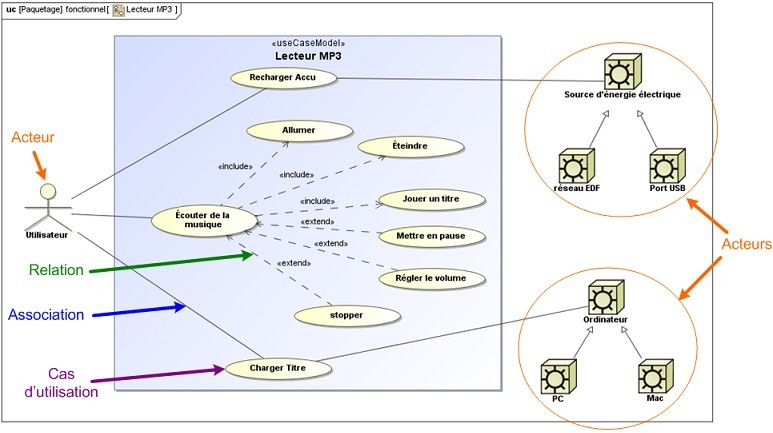
\includegraphics[width=0.8\linewidth]{image1.png}
	\caption{Diagramme des cas d'utilisation d'un lecteur MP3 (partiel)}

\end{figure}

\noindent \begin{flushleft}
	
	
	\begin{figure}[H]
		\centering
		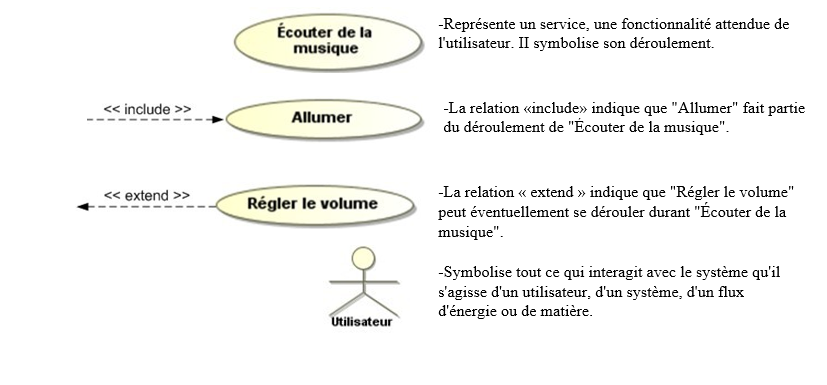
\includegraphics[width=0.8\linewidth]{Capture.png}
	\end{figure}
	
	Un cas d'utilisation repr\'{e}sente les interactions entre un acteur et le syst\`{e}me d'un point de vue « boite noire », et comprend l'ensemble des sc\'{e}narios identifi\'{e}s (nominal, alternatifs, et d'erreurs). Ces sc\'{e}narios peuvent \^{e}tre d\'{e}taill\'{e}s par une description textuelle et/ou par un diagramme de s\'{e}quence.
	
	\noindent 
\end{flushleft}


\subsubsection{ Le diagramme des exigences}

\noindent \begin{flushleft}
	
	
	Que ce soit pour l'ing\'{e}nierie syst\`{e}me ou pour des r\'{e}alisations logicielles, les exigences sont couramment utilis\'{e}es pour formaliser les pr\'{e}requis du syst\`{e}me, se traduisant par des fonctionnalit\'{e}s ou conditions qui doivent ou devraient \^{e}tre satisfaites par le syst\`{e}me (selon les \'{e}ventuelles priorit\'{e}s associ\'{e}es aux exigences).
	
	Pour la ma\^{i}trise d'ouvrage (MOA), les exigences ont pour objectif d'assurer l'ad\'{e}quation de la solution (le syst\`{e}me r\'{e}alis\'{e}) avec les besoins. Les exigences peuvent \^{e}tre formalis\'{e}es et cat\'{e}goris\'{e}es par centre d'int\'{e}r\^{e}ts ou aspects, par exemple diff\'{e}renciant les exigences fonctionnelles des exigences techniques (performance, fiabilit\'{e}, ergonomie, etc.).
	
	\noindent La formalisation des exigences peut \^{e}tre effectu\'{e}e avec une feuille Excel, ou avec un outil sp\'{e}cialis\'{e} tel que DOORS ou CaliberRM. L'int\'{e}r\^{e}t qu'offrent ces outils est la gestion des exigences dans une organisation structur\'{e}e. Les exigences sont \'{e}galement utilis\'{e}es pour la mod\'{e}lisation, par la cr\'{e}ation d'associations entre exigences et cas d'utilisations, blocs ou tout type d'\'{e}l\'{e}ment du mod\`{e}le, \'{e}tablissant une tra\c{c}abilit\'{e}. Il est possible avec l'outil Enterprise Architect de d\'{e}finir les exigences ou d\`{e}s les importer depuis un outil tel que DOORS, et de les associer avec les \'{e}l\'{e}ments du mod\`{e}le.
	
	\noindent SysML formalise les exigences et leur repr\'{e}sentation, s'inspirant des fonctionnalit\'{e}s des outils actuellement disponibles sur le march\'{e}, par exemple EA, DOORS, CaliberRM. Ainsi SysML d\'{e}finit une repr\'{e}sentation graphique et visuelle des exigences textuelles, permet une organisation hi\'{e}rarchique et l'association avec les \'{e}l\'{e}ments du mod\`{e}le.
	
	\noindent 
	
	\noindent SysML d\'{e}finit de nouveaux types de d'associations (liens de d\'{e}pendance st\'{e}r\'{e}otyp\'{e}s) :
\end{flushleft}

\begin{enumerate}
	\item  Derive : une ou plusieurs exigences sont d\'{e}riv\'{e}es d'une exigence
	
	\item  Satisfy: un ou plusieurs \'{e}l\'{e}ments du mod\`{e}le (par exemple un bloc) permettent de satisfaire une exigence
	
	\item  Verify: un ou plusieurs \'{e}l\'{e}ments du mod\`{e}le (par exemple un « test case ») permettent de v\'{e}rifier et valider une exigence
	
	\item  Refine: un ou plusieurs \'{e}l\'{e}ments du mod\`{e}le, par exemple un cas d'utilisation, red\'{e}finit une exigence
	
	\item  SysML d\'{e}finit de nouveaux commentaires st\'{e}r\'{e}otyp\'{e}s permettant d'associer une explication \`{a} des associations ou \'{e}l\'{e}ments du mod\`{e}le :
	
	\item  Problem: commentaire dont la description pose le probl\`{e}me ou le besoin qui a donn\'{e} lieu \`{a} la cr\'{e}ation de l'association ou de l'\'{e}l\'{e}ment associ\'{e}
	
	\item  Rationale: commentaire dont la description indique la raison ou la justification par rapport \`{a} l'\'{e}l\'{e}ment ou l'association associ\'{e}
\end{enumerate}

\noindent \begin{flushleft}
	
	
	\noindent Exemple d'associations et de commentaires des sp\'{e}cifications officielles de SysML (OMG) : 
\end{flushleft}


\begin{figure}[H]
	\centering
	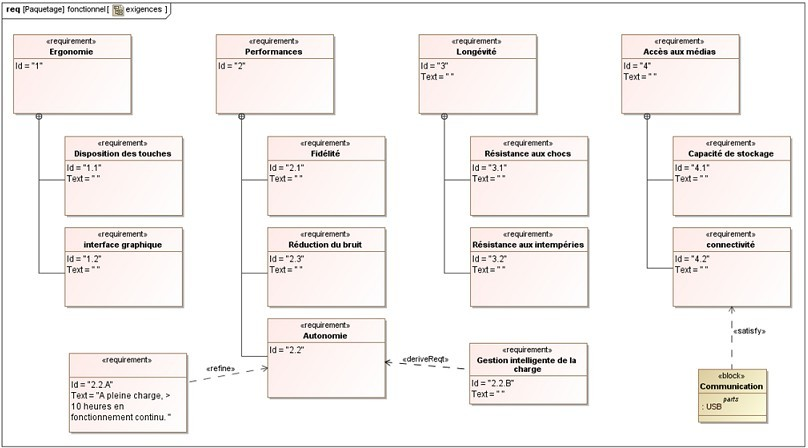
\includegraphics[width=0.8\linewidth]{image6.png}
	\caption{Diagramme d'exigence partiel d'un lecteur MP3}
	
\end{figure}

\noindent \textbf{}


\noindent \begin{flushleft}
	
	
	\noindent 
	
	\noindent 
	
	\noindent 
	
	\noindent 
	
	\noindent 
	
	\noindent 
	\begin{figure}[H]
		\centering
		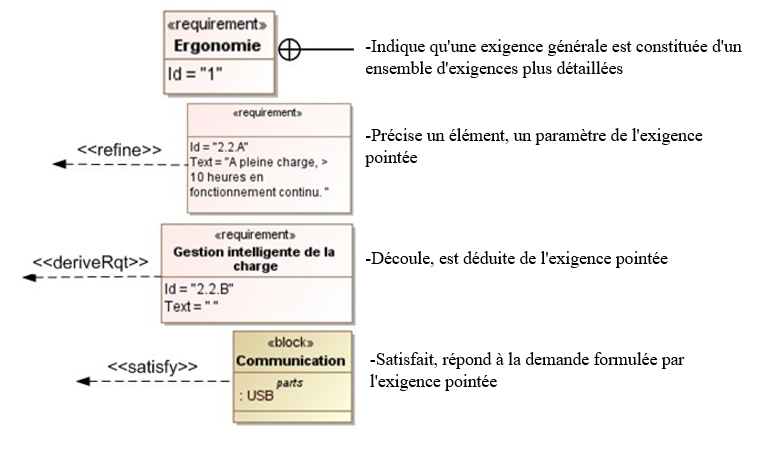
\includegraphics[width=0.8\linewidth]{Capture2.png}
		
	\end{figure}
	
	\noindent 
	
	\noindent 
	
	\noindent 
	
	\noindent 
	
	\noindent 
	
	\noindent 
	
	\noindent 
	
	\noindent 
	
	\noindent 
	
	\noindent 
	
	\noindent 
	
	\noindent 
	
	\noindent 
\end{flushleft}


\subsubsection{ Le diagramme de contexte}

\noindent \begin{flushleft}
	Il compl\`{e}te \'{e}ventuellement la description fonctionnelle en pr\'{e}sentant tous les \'{e}l\'{e}ments externes qui influencent le syst\`{e}me \'{e}tudi\'{e} et le syst\`{e}me lui-m\^{e}me.
	
	\noindent 
\end{flushleft}

\begin{figure}[H]
	\centering
	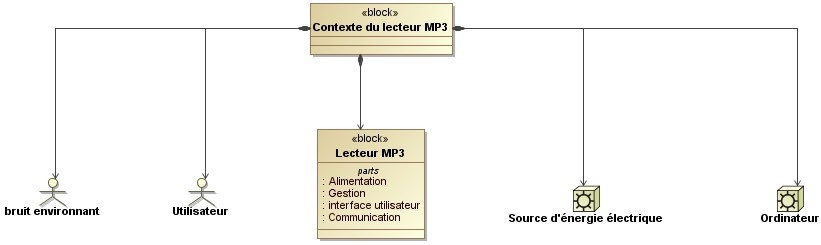
\includegraphics[width=0.8\linewidth]{image11.png}
	\caption{Diagramme de contexte d'un lecteur MP3}
	
\end{figure}

\noindent \begin{flushleft}
	
\end{flushleft}


\subsection{ Description structurelle}

\noindent \begin{flushleft}
	Le langage sysML propose 2 diagrammes destin\'{e}s \`{a} d\'{e}crire la composition du syst\`{e}me.
\end{flushleft}


\subsubsection{ Le diagramme de d\'{e}finition des blocks (BDD)}

\noindent \begin{flushleft}
	Le diagramme de d\'{e}finition de bloc (BDD, ou Block Definition Diagram en anglais) repr\'{e}sente la vue bo\^{i}te noire d'un bloc. Ainsi le bloc principal et la hi\'{e}rarchie des blocs qui le composent, qu'ils soient logiciels ou mat\'{e}riels, sont sp\'{e}cifi\'{e}s dans ce diagramme.
	
	\noindent Par rapport \`{a} UML, le BDD de SysML red\'{e}finit le diagramme de classe en rempla\c{c}ant les classes par des blocs.
	
	\noindent Le BDD est similaire \`{a} la premi\`{e}re page d'une notice de montage d'un meuble, indiquant la liste des \'{e}l\'{e}ments et des pi\`{e}ces \`{a} assembler avec leurs quantit\'{e}s respectives.
	
	\noindent Il r\'{e}pertorie les constituants du syst\`{e}me ou d'un block en pr\'{e}cisant \'{e}ventuellement leur r\^{o}le et leur quantit\'{e}. Chaque block peut faire l'objet d'une description plus pr\'{e}cise en indiquant ses constituants, ses propri\'{e}t\'{e}s, les op\'{e}rations qu'il peut effectuer ainsi que les contraintes ou limites auxquelles il est soumis. Exemple : 
	
	\noindent 
\end{flushleft}

\begin{figure}[H]
	\centering
	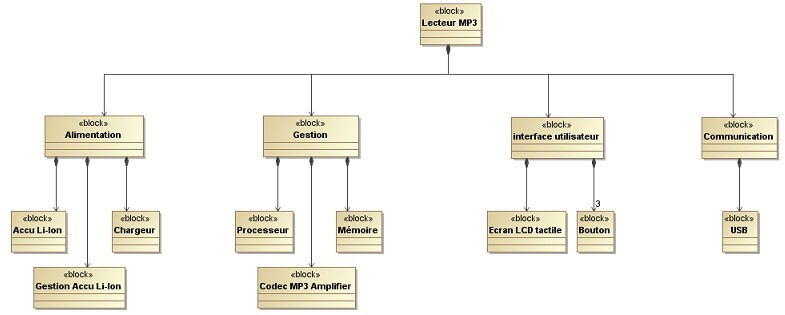
\includegraphics[width=0.8\linewidth]{image12.png}
	\caption{Diagramme de d\'{e}finition de blocks d'un lecteur MP3}
	
\end{figure}

\noindent \begin{flushleft}
	
	
	\noindent Remarque : Dans le cas pr\'{e}sent, Le lecteur MP3 dispose d'une interface utilisateur constitu\'{e}e d'un \'{e}cran LCD tactile et de 3 boutons.
\end{flushleft}


\subsubsection{ Le diagramme de block interne (IBD)}

\noindent \begin{flushleft}
	Le diagramme de bloc interne (IBD, ou Internal Block Diagram) d\'{e}crit la vue interne d'un bloc ou vue bo\^{i}te blanche, et se base sur le BDD pour assembler les blocs qui composent le bloc principal. Il repr\'{e}sente les liens, les flux et les informations \'{e}chang\'{e}es entre les part d'un block ou du syst\`{e}me. Le cadre du diagramme repr\'{e}sente le block lui m\^{e}me ou le syst\`{e}me.
	
	\noindent Le bloc principal peut \^{e}tre repr\'{e}sent\'{e} comme conteneur sur l'IBD ou \^{e}tre absent de ce diagramme. Les blocs qui le composent, d\'{e}finis dans le BDD, sont instanci\'{e}s en parties (tout comme les parties dans un diagramme de structure composite avec UML2). Ces parties sont assembl\'{e}es par des connecteurs qui relient leurs ports (ports standards avec interfaces expos\'{e}es et/ou ports de flux).
	
	\noindent Il est \'{e}galement possible de relier des parties directement entre elles, l'utilisation des ports \'{e}tant optionnelle.
	
	\noindent Par rapport \`{a} UML2, l'IBD de SysML red\'{e}finit le diagramme de structure composite en ajoutant entre autre les ports de flux (« flow ports » en anglais). 
	
\end{flushleft}
\begin{figure}[H]
	\centering
	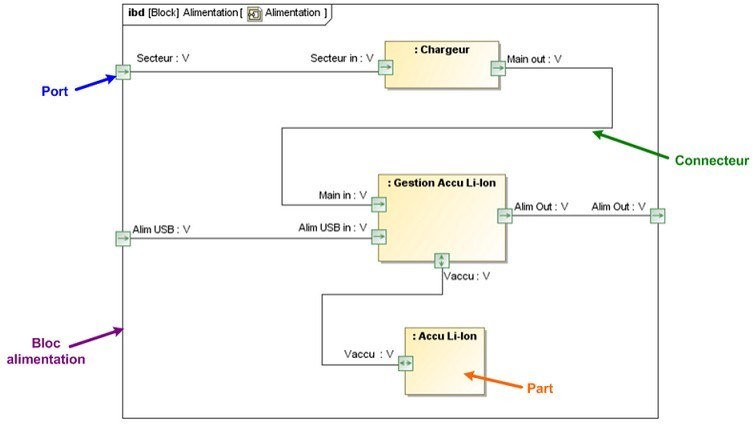
\includegraphics[width=0.8\linewidth]{image13.png}
	\caption{Diagramme de block interne du Block Alimentation (Lecteur MP3)}
	
\end{figure}

\noindent \begin{flushleft}
	
	
	\noindent Un port symbolise ce qui peut entrer/sortir d'un block. On en distingue 2 types :
	
	\noindent 
	
	\noindent -Le port de flux (flow port) \includegraphics*[bb=0 0 0.21in 0.20in, width=0.21in, height=0.20in, keepaspectratio=false]{image14} qui correspond \`{a} l'entr\'{e}e/sortie d'un flux de mati\`{e}re, d'\'{e}nergie, de donn\'{e}es, etc. Le sens de circulation peut \^{e}tre pr\'{e}cis\'{e} par une fl\`{e}che.
	
	\noindent -Le port standard  \includegraphics*[bb=0 0 0.21in 0.20in, width=0.21in, height=0.20in, keepaspectratio=false]{image15} qui repr\'{e}sente un point de communication li\'{e} \`{a} un service :
\end{flushleft}

\begin{enumerate}
	\item  une entr\'{e}e/sortie v\'{e}hiculant des informations (ou des ordres) logiques/num\'{e}riques comme l'\'{e}tat d'un bouton poussoir ;
	
	\item  une communication plus \'{e}labor\'{e}e entre 2 parts via un r\'{e}seau.
\end{enumerate}

\noindent \begin{flushleft}
	Les connecteurs repr\'{e}sentent les liaisons entre les ports ou les parts, en pr\'{e}cisant \'{e}ventuellement la nature du lien ou ce qui est r\'{e}ellement v\'{e}hicul\'{e}.
\end{flushleft}


\subsubsection{ Le diagramme param\'{e}trique}

\noindent \begin{flushleft}
	Le diagramme param\'{e}trique est une nouveaut\'{e} SysML qui red\'{e}finit le diagramme interne de bloc SysML (lui-m\^{e}me bas\'{e} sur le diagramme de structure composite UML2), et permet d'int\'{e}grer des analyses syst\`{e}mes (performance, fiabilit\'{e}, etc.) avec des blocs de contrainte.
	
	\noindent Un bloc de contrainte repr\'{e}sente une expression math\'{e}matique dont les param\`{e}tres peuvent faire r\'{e}f\'{e}rence \`{a} des \'{e}l\'{e}ments du syst\`{e}me, par exemple des propri\'{e}t\'{e}s de blocs.
	
	\noindent Exemples de blocs de contraintes : $\mathrm{\{}$F=m*a$\mathrm{\}}$, $\mathrm{\{}$a=dv/dt$\mathrm{\}}$
	
	\noindent Dans un premier temps, de fa\c{c}on similaire \`{a} la cr\'{e}ation du diagramme BDD, les blocs de contraintes sont d\'{e}finis dans un diagramme de classe, et repr\'{e}sent\'{e}s comme suit :
	
	\noindent 
	
	\begin{figure}[h]
		\centering
		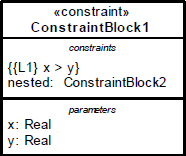
\includegraphics[width=0.4\linewidth]{image16.png}
	\end{figure}
	
	
	
	\noindent Apr\`{e}s avoir d\'{e}fini les blocs de contrainte, il faut g\'{e}n\'{e}rer un diagramme param\'{e}trique :
	
	\noindent Des blocs de contraintes sont instanci\'{e}s, donnant lieu aux propri\'{e}t\'{e}s de contrainte (ou constraint property), h\'{e}ritant ainsi des param\`{e}tres du bloc de contrainte (note : il n'y a pas de diff\'{e}renciation entre param\`{e}tres d'entr\'{e}e et param\`{e}tres de sortie)
	
	\noindent Des propri\'{e}t\'{e}s syst\`{e}mes (optionnellement li\'{e}es \`{a} des blocs)
	
	\noindent Des connecteurs reliant les propri\'{e}t\'{e}s syst\`{e}mes aux param\`{e}tres des propri\'{e}t\'{e}s de contrainte, ou reliant uniquement des param\`{e}tres des propri\'{e}t\'{e}s de contrainte
\end{flushleft}


\begin{figure}[H]
	\centering
	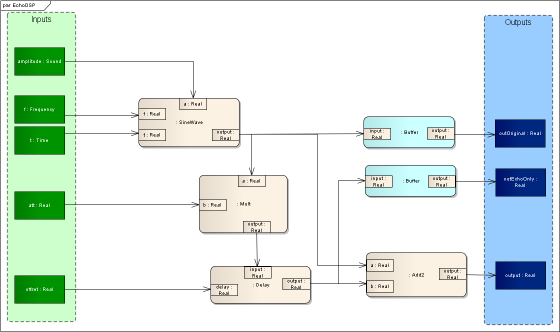
\includegraphics[width=0.8\linewidth]{image17.png}
	\caption{Diagramme paramétrique d'un lecteur MP3}
	
\end{figure}

\noindent \begin{flushleft}
	
\end{flushleft}

\noindent \begin{enumerate}
	\item \begin{enumerate}
		\item Informations li\'{e}es au diagramme param\'{e}trique :
	\end{enumerate}
\end{enumerate}

\noindent \begin{flushleft}
	Le diagramme comporte six propri\'{e}t\'{e}s de contrainte, dont deux propri\'{e}t\'{e}s instanci\'{e}es du m\^{e}me bloc de contrainte : Buffer.
	
	\noindent Les param\`{e}tres syst\`{e}mes sont cat\'{e}goris\'{e}s entre entr\'{e}es et sorties (ex : amplitude et fr\'{e}quence en entr\'{e}e, output en sortie). Ces param\`{e}tres sont associ\'{e}s aux param\`{e}tres de propri\'{e}t\'{e}s de contrainte (par exemple la fr\'{e}quence d'entr\'{e}e f est reli\'{e}e au param\`{e}tre f de la propri\'{e}t\'{e} de contrainte SineWave)
	
	\noindent Certaines propri\'{e}t\'{e}s de contrainte sont reli\'{e}es entre elle (ex : le param\`{e}tre SineWave.output est reli\'{e} \`{a} Buffer.input et \`{a} Add.a)
	
	\noindent Avec certains outils, ce diagramme peut \^{e}tre ex\'{e}cut\'{e} dans le cadre de simulation du syst\`{e}me.
	
	\noindent Il est possible sous Enterprise Architect de saisir des expressions pour chacun des blocs de contraintes (par exemple en VBScript ou JavaScript), ainsi que de renseigner diff\'{e}rentes valeurs pour les param\`{e}tres syst\`{e}mes. Ces expressions et valeurs peuvent \^{e}tre alors ex\'{e}cut\'{e}es par le module de simulation Enterprise Architect comme illustr\'{e} ci-dessous~:
\end{flushleft}
\noindent 


\begin{figure}[H]
	\centering
	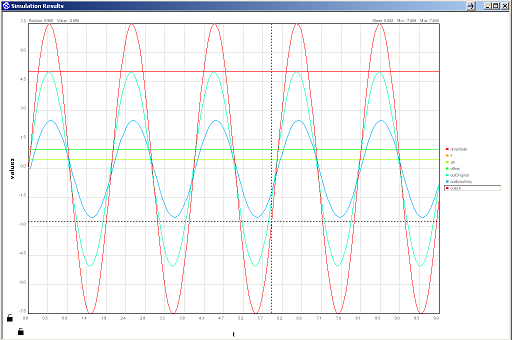
\includegraphics[width=0.8\linewidth]{image18.png}
	
	
\end{figure}

\noindent \begin{flushleft}
	
	
	\noindent Value Types
	
	\noindent Les Value Types sont une nouveaut\'{e} SysML pour d\'{e}finir des types de valeurs r\'{e}utilisables pour des propri\'{e}t\'{e}s du mod\`{e}le, par exemple des blocs. De fa\c{c}on similaire \`{a} la mod\'{e}lisation UML o\`{u} les attributs de classes peuvent \^{e}tre typ\'{e}s par d'autres classes, SysML permet de d\'{e}finir des propri\'{e}t\'{e}s de blocs typ\'{e}es avec des Value Type.
	
	\noindent La Value Type a la particularit\'{e} de contenir 2 propri\'{e}t\'{e}s optionnelles : une unit\'{e} et une dimension. Les unit\'{e}s et dimensions sont des classes sp\'{e}cialis\'{e}es et d\'{e}finies dans le mod\`{e}le, par exemple :
	
	\begin{figure}[H]
		\centering
		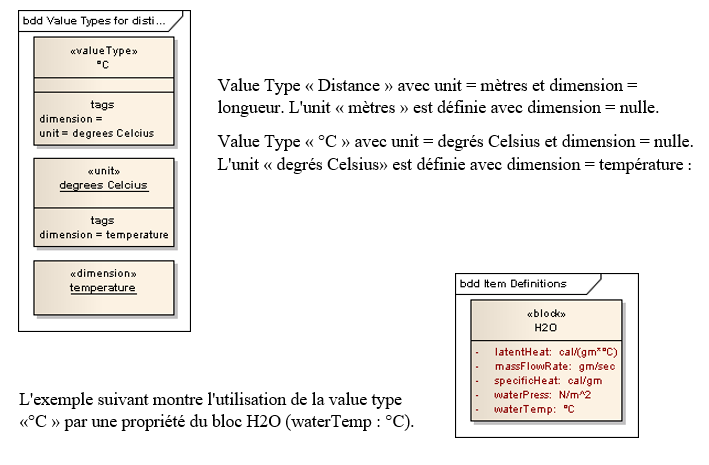
\includegraphics[width=0.8\linewidth]{Capture3.png}
		
	\end{figure}
	
	\newpage
	
\end{flushleft}


\subsection{ Description comportementale}

\noindent \begin{flushleft}
	Pour mod\'{e}liser l'aspect dynamique d'un syst\`{e}me et/ou de ses constituants, le langage sysML propose des diagrammes de comportement parmi lesquels on trouve :
\end{flushleft}


\subsubsection{ Le diagramme de s\'{e}quence (sd)}

\noindent \begin{flushleft}
	Le diagramme de s\'{e}quence repr\'{e}sente les \'{e}l\'{e}ments intervenant dans le sc\'{e}nario, ainsi que les \'{e}changes de messages entre le syst\`{e}me et des acteurs, ou entre des parties du syst\`{e}me, de mani\`{e}re chronologique en pr\'{e}cisant d'\'{e}ventuelles contraintes de temps. La lecture d'un tel diagramme se fait de haut en bas.
	
	\noindent Dans un premier temps, on peut choisir de repr\'{e}senter les interactions entre l'acteur et le syst\`{e}me (vue boite noire). Par la suite il est possible de rentrer en d\'{e}tails avec un diagramme de s\'{e}quence qui repr\'{e}sente les blocs internes du syst\`{e}me intervenant dans un sc\'{e}nario (pour un message \'{e}mis par l'acteur, le diagramme d\'{e}crit l'encha\^{i}nement des messages \'{e}chang\'{e}s entre les blocs internes du syst\`{e}me) ; on parle ainsi de la vue boite blanche (comportement du syst\`{e}me).
	
	\noindent Les \'{e}l\'{e}ments intervenant sont repr\'{e}sent\'{e}s par des lignes de vie (lifetime en anglais).
	
	\noindent Ces lignes de vies peuvent \^{e}tre des instances de blocs, \'{e}tablissant un lien avec la mod\'{e}lisation structurelle du syst\`{e}me, permettant ainsi d'\'{e}tablir une coh\'{e}rence dans le mod\`{e}le :
	
	\noindent 
	
	\noindent On peut acc\'{e}der aux propri\'{e}t\'{e}s du bloc d'une ligne de vie (et \'{e}galement aux diagrammes de
	
	\noindent BDD et d'IBD de ce bloc)
	
	Chaque message \'{e}chang\'{e} peut \^{e}tre utilis\'{e} pour l'identification des op\'{e}rations de blocs
	
	\noindent L'ensemble des propri\'{e}t\'{e}s du diagramme de s\'{e}quence utilis\'{e}es en UML sont \'{e}galement disponibles avec SysML : messages synchrones ou asynchrones, op\'{e}rateurs (ex : alt, loop, opt, par), r\'{e}f\'{e}rences vers d'autres diagrammes de s\'{e}quence (ex : naviguer de la vue boite noire du sc\'{e}nario vers la vue boite blanche), etc. 
\end{flushleft}


\begin{figure}[H]
	\centering
	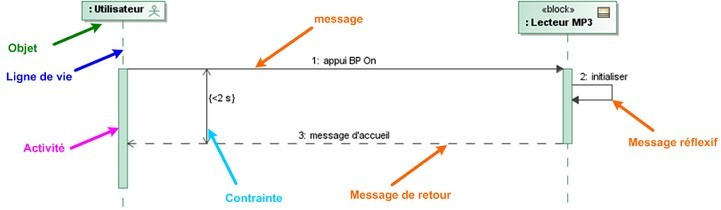
\includegraphics[width=0.8\linewidth]{image21.png}
	\caption{Diagramme de s\'{e}quence du cas d'utilisation "Allumer" du lecteur MP3}
	
\end{figure}
\newpage

\begin{figure}[H]
	\centering
	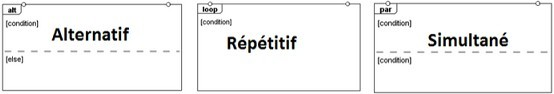
\includegraphics[width=0.8\linewidth]{image22.png}
	
	
\end{figure}
\noindent \begin{flushleft}
	Lorsque une s\'{e}quence de message n'est pas lin\'{e}aire (conditionnelle, r\'{e}p\'{e}titive, simultan\'{e}e), les messages concern\'{e}s sont encadr\'{e}s par des fragments combin\'{e}s :
	
	\noindent 
\end{flushleft}



\subsubsection{ Le diagramme d'activit\'{e}}

\begin{flushleft}
	Le diagramme d'activit\'{e} est utilis\'{e} pour repr\'{e}senter les \'{e}tapes d'un traitement. Avec SysML, les « input et output pins » sont particuli\`{e}rement utilis\'{e}s pour repr\'{e}senter le type d'\'{e}l\'{e}ment qui est requis en entr\'{e}e d'une activit\'{e} ou action, et ce qui est g\'{e}n\'{e}r\'{e} en sortie.
	
	\noindent 
	\noindent \begin{center}
		\includegraphics*[bb=0 0 3.18in 2.78in, width=3.18in, height=2.78in, keepaspectratio=false]{image23}
		
	\end{center}
	
	Si une action ou activit\'{e} repr\'{e}sente l'op\'{e}ration d'un bloc, on peut garantir la coh\'{e}rence du mod\`{e}le en s'assurant que ce qui est d\'{e}fini en entr\'{e}e d'une activit\'{e} corresponde \`{a} la signature de l'op\'{e}ration du bloc ou de son interface.
	
	\noindent Toutes les propri\'{e}t\'{e}s des diagrammes d'activit\'{e}s UML sont \'{e}galement disponibles avec SysML. SysML a rajout\'{e} quelques sp\'{e}cificit\'{e}s :
\end{flushleft}

\begin{enumerate}
	\item  Notion de contr\^{o}le pour activer ou d\'{e}sactiver les actions en cours.
	
	\item  Sp\'{e}cification de la nature du d\'{e}bit sur le flot : syst\`{e}me continu ou discret
	
	\item  D\'{e}finition de taux et de probabilit\'{e} sur les flots
\end{enumerate}


\subsubsection{ Le diagramme d'\'{e}tat (stm)}

\noindent \begin{flushleft}
	
	
	\noindent Le diagramme d'\'{e}tats est utilis\'{e} avec SysML de la m\^{e}me mani\`{e}re qu'avec UML2, c'est-\`{a}-dire qu'il permet de repr\'{e}senter le cycle de vie auquel doivent se conformer toutes les instances d'un bloc donn\'{e}, ce au travers de la mod\'{e}lisation de tous les \'{e}tats possibles. Il mod\'{e}lise l'\'{e}volution de l'\'{e}tat d'un block en fonction des \'{e}v\'{e}nements qui peuvent se produire.
	
	\noindent Seuls les blocs qui sont importants d'un point de vue m\'{e}tier, ou qui sont de nature complexe, poss\`{e}dent un diagramme d'\'{e}tat. Exemple : 
\end{flushleft}


\begin{figure}[H]
	\centering
	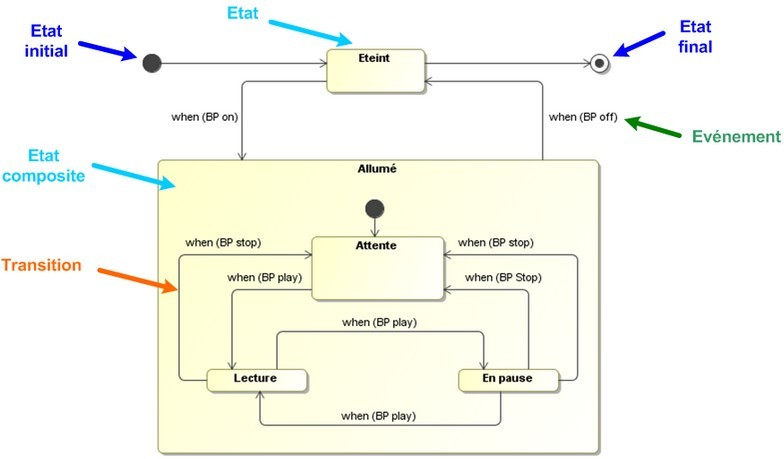
\includegraphics[width=0.8\linewidth]{image24.png}
	\caption{Diagramme \'{e}tat - transition partiel d'un lecteur MP3}
	
\end{figure}

\noindent \begin{flushleft}
	Les propri\'{e}t\'{e}s du diagramme d'\'{e}tat UML sont \'{e}galement disponibles avec SysML : conditions sur \'{e}v\'{e}nements, effets, activit\'{e} durable, transitions, \'{e}tats composites, modularit\'{e}, r\'{e}gions concurrentes, etc.
	
	\noindent 
\end{flushleft}


\section{ Approche SysML}

\noindent \begin{flushleft}
	
	\begin{figure}[H]
		\centering
		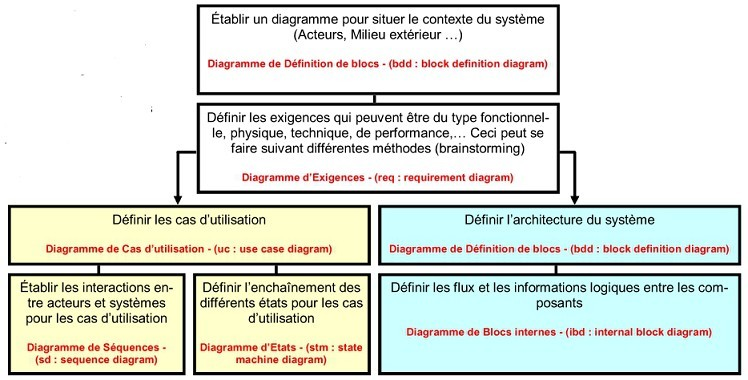
\includegraphics[width=0.8\linewidth]{image25.png}
		\caption{}
		
	\end{figure}
	
	Le SysML est un langage et non une m\'{e}thode. Il est n\'{e}anmoins possible d'\'{e}tablir un ordre pour comprendre et expliquer le fonctionnement des syst\`{e}mes.
	
	\noindent 
	
	\noindent 
	
	\noindent 
	
	\noindent 
	
	\noindent 
	
	\noindent 
\end{flushleft}


\section{ La relation entre UML et SysML}

\noindent \begin{flushleft}
	
	
	\noindent SysML r\'{e}utilise un sous-ensemble de UML 2.1, appel\'{e} ''UML4SysML'', qui repr\'{e}sente environ la moiti\'{e} du langage UML. Une partie importante de l'UML des concepts ont \'{e}t\'{e} \'{e}cart\'{e}s car ils n'\'{e}taient pas consid\'{e}r\'{e}s comme pertinents pour les besoins du mod\`{e}le de SE. Certains des diagrammes r\'{e}utilis\'{e}s ont \'{e}t\'{e} inclus comme dans UML 2.1.1 . Ceux-ci incluent la machine d'\'{e}tat, la s\'{e}quence et les diagrammes de cas d'utilisation. D'autres diagrammes ont \'{e}t\'{e} \'{e}tendus, tels que les diagrammes d'activit\'{e}, afin de r\'{e}pondre aux besoins sp\'{e}cifiques 32 des SE. De plus, SysML a omis certains diagrammes UML, \`{a} savoir d'objet, de composant, de d\'{e}ploiement, de communication, de temps et d'interactions. Les diagrammes de structure dont diagramme de Classe et composition ont \'{e}t\'{e} fondamentalement modifi\'{e}s et remplac\'{e}s par des diagrammes de d\'{e}finition de blocs et diagrammes de blocs internes. Ces extensions sont bas\'{e}es sur le m\'{e}canisme de profilage UML standard, qui inclut les st\'{e}r\'{e}otypes UML, extensions de diagramme UML et la biblioth\`{e}que de mod\`{e}les. Le m\'{e}canisme de profilage a \'{e}t\'{e} choisi sur d'autres m\'{e}canismes d'extension afin de tirer parti des outils existants bas\'{e}s sur UML pour la mod\'{e}lisation de syst\`{e}mes. En outre, SysML ajoute deux nouveaux diagrammes, ceux-ci \'{e}tant diagrammes d'exigences et diagrammes param\'{e}triques, et int\'{e}gr\'{e} de nouvelles capacit\'{e}s de sp\'{e}cification liens tels que l'allocation
	
	\noindent 
	
	\noindent 
\end{flushleft}


\begin{figure}[H]
	\centering
	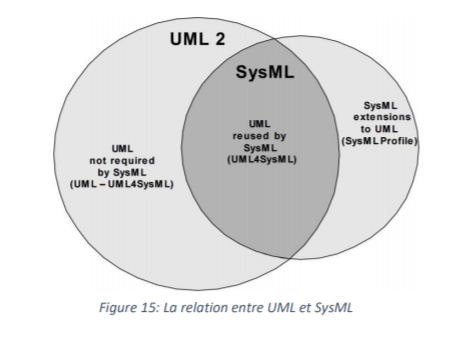
\includegraphics[width=0.8\linewidth]{image26.png}
	\caption{Relation entre uml et sysml}
	
\end{figure}


\noindent \begin{flushleft}
	
\end{flushleft}


\section{ Synthèse: }

\noindent \begin{flushleft}
	
	
	\noindent Dans cette section, nous avons mis en \'{e}vidence les points suivants :
	
	\noindent 1. SysML permet de mod\'{e}liser un produit et son environnement par un syst\`{e}me, c'est-\`{a}-dire un ensemble de composants qui interagissent entre eux. 
	
	\noindent 2. Cette mod\'{e}lisation est multipoints de vue et inclut notamment des aspects fonctionnels, structurels et comportementaux. 3. Un mod\`{e}le SysML est repr\'{e}sent\'{e} par un ensemble de bo\^{i}tes et de lignes, munies de types, de nom permettant de les identifier, et d'une hi\'{e}rarchie (une bo\^{i}te contient d'autres bo\^{i}tes et des lignes).
	
	\noindent 4. Les bo\^{i}tes et les lignes sont assembl\'{e}es au sein de diagrammes interd\'{e}pendants : un m\^{e}me \'{e}l\'{e}ment, rep\'{e}r\'{e} par son nom, peut figurer sur des diagrammes diff\'{e}rents, qui apportent alors des informations compl\'{e}mentaires.
	
	\noindent 5. Il existe neuf types de diagrammes. Ces types, ainsi que les relations possibles entre les \'{e}l\'{e}ments repr\'{e}sent\'{e}s par ces diagrammes, sont r\'{e}capitul\'{e}s sur la figure 14 (le diagramme des paquets a \'{e}t\'{e} omis dans un souci de simplicit\'{e}). 6. Un diagramme doit toujours repr\'{e}senter l'int\'{e}rieur d'une bo\^{i}te. Cependant, cette repr\'{e}sentation peut \^{e}tre partielle (on ne repr\'{e}sente que ce dont on a besoin)
	
	\noindent 
\end{flushleft}


\subsection{Le processus unifie UP (Unified Process)}

\noindent \begin{flushleft}
	Le processus unifi\'{e} not\'{e} UP est un processus de d\'{e}veloppement logiciel moderne, tr\`{e}s complet et construit sur UML. Il est it\'{e}ratif, centr\'{e} sur l'architecture, pilot\'{e} par des cas d'utilisation et orient\'{e} vers la diminution des risques. Il regroupe les activit\'{e}s \`{a} mener pour transformer les besoins d'un utilisateur en syst\`{e}me logiciel 
	
	\noindent C'est un patron de processus pouvant \^{e}tre adapt\'{e} \`{a} une large classe de syst\`{e}mes logiciels, \`{a} diff\'{e}rents domaines d'application, \`{a} diff\'{e}rents types d'entreprises, \`{a} diff\'{e}rents niveaux de comp\'{e}tences et \`{a} diff\'{e}rentes tailles de l'entreprise.
\end{flushleft}


\subsubsection{ UP est it\'{e}ratif}

\noindent \begin{flushleft}
	L'it\'{e}ration est une r\'{e}p\'{e}tition d'une s\'{e}quence d'instructions ou d'une partie de programme un nombre de fois fix\'{e} \`{a} l'avance ou tant qu'une condition d\'{e}finie n'est pas remplie, dans le but de reprendre un traitement sur des donn\'{e}es diff\'{e}rentes.
	
	\noindent Elle qualifie un traitement ou une proc\'{e}dure qui ex\'{e}cute un groupe d'op\'{e}rations de fa\c{c}on r\'{e}p\'{e}titive jusqu'\`{a} ce qu'une condition bien d\'{e}finie soit remplie.
	
	\noindent 
\end{flushleft}


\begin{figure}[H]
	\centering
	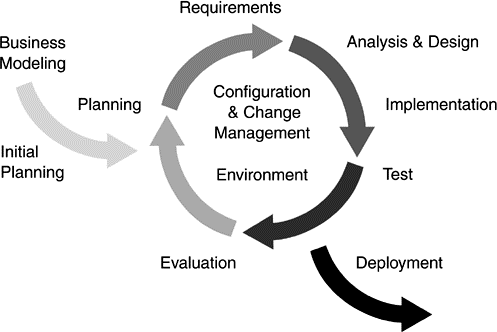
\includegraphics[width=0.8\linewidth]{image27.png}
	\caption{UP est it\'{e}ratif}
	
\end{figure}

\noindent \begin{flushleft}
	
	
	\noindent Une it\'{e}ration prend en compte un certain nombre de cas d'utilisation et traite en priorit\'{e} les risques majeurs.
\end{flushleft}


\subsubsection{ UP est centr\'{e} sur l'architecture}

\noindent \begin{flushleft}
	D\`{e}s le d\'{e}marrage du processus, on aura une vue sur l'architecture \`{a} mettre en place.
	
	\noindent L'architecture d'un syst\`{e}me logiciel peut \^{e}tre d\'{e}crite comme les diff\'{e}rentes vues du syst\`{e}me qui doit \^{e}tre construit. L'architecture logicielle \'{e}quivaut aux aspects statiques et dynamiques les plus significatifs du syst\`{e}me. L'architecture \'{e}merge des besoins de l'entreprise, tels qu'ils sont exprim\'{e}s par les utilisateurs et autres intervenants et tels qu'ils sont refl\'{e}t\'{e}s par les cas d'utilisation .
\end{flushleft}


\begin{figure}[H]
	\centering
	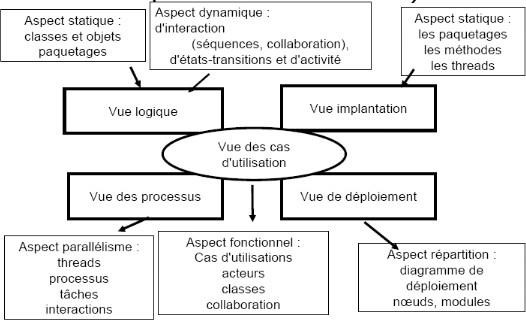
\includegraphics[width=0.8\linewidth]{image28.png}
	\caption{UP est centr\'{e} sur l'architecture}
	
\end{figure}


\noindent \begin{flushleft}
	
\end{flushleft}


\subsubsection{ UP est pilot\'{e} par les cas d'utilisation}

\noindent \begin{flushleft}
	Le but principal d'un syst\`{e}me informatique est de satisfaire les besoins du client. Le processus de d\'{e}veloppement sera donc ax\'{e} sur l'utilisateur. Les cas d'utilisation permettent d'illustrer ces besoins.
	
	\noindent Ils d\'{e}tectent puis d\'{e}crivent les besoins fonctionnels (du point de vue de l'utilisateur), et leur ensemble constitue le mod\`{e}le de cas d'utilisation qui dicte les fonctionnalit\'{e}s compl\`{e}tes du syst\`{e}me.
\end{flushleft}


\begin{figure}[H]
	\centering
	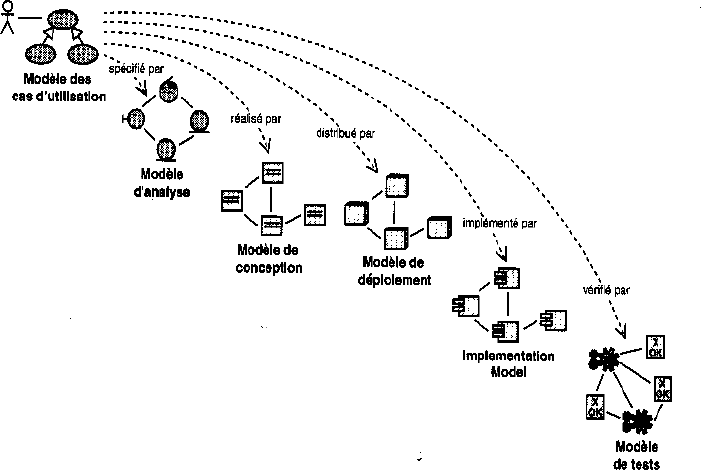
\includegraphics[width=0.8\linewidth]{image29.png}
	\caption{UP est pilot\'{e} par les cas d'utilisation}
	
\end{figure}

\subsubsection{ Les activit\'{e}s}

\noindent \begin{flushleft}
	Expression des besoins : permet de d\'{e}finir les diff\'{e}rents besoins :
\end{flushleft}

\begin{enumerate}
	\item  Besoins principaux et fournir une liste de leurs fonctions.
	
	\item  Besoins fonctionnels du point de vue de l'utilisateur.
	
	\item  Besoins non fonctionnels ou technique.
\end{enumerate}

\noindent \begin{flushleft}
	
	
	\noindent 
	
	\noindent Analyse : Un mod\`{e}le d'analyse livre une sp\'{e}cification compl\`{e}te des besoins issus des cas d'utilisation et les structure sous une forme qui facilite :
\end{flushleft}

\begin{enumerate}
	\item  La compr\'{e}hension (sc\'{e}narios).
	
	\item  La pr\'{e}paration (d\'{e}finition de l'architecture).
	
	\item  La modification et la maintenance du futur syst\`{e}me.
\end{enumerate}

\noindent \begin{flushleft}
	
	
	\noindent 
	
	\noindent Conception :
\end{flushleft}

\begin{enumerate}
	\item  Elle d\'{e}termine les principales interfaces et les transcrit \`{a} l'aide d'une notation commune.
	
	\item  Elle constitue un point de d\'{e}part \`{a} l'impl\'{e}mentation :
	
	\item  Elle d\'{e}compose le travail d'impl\'{e}mentation en sous-syst\`{e}me
	
	\item  Elle cr\'{e}\'{e}e une abstraction transparente de l'impl\'{e}mentation
\end{enumerate}

\noindent \begin{flushleft}
	
	
	\noindent Impl\'{e}mentation : Les objectifs principaux de l'impl\'{e}mentation sont :
\end{flushleft}

\begin{enumerate}
	\item  Planifier les int\'{e}grations des composants pour chaque it\'{e}ration.
	
	\item  Produire les classes et les sous-syst\`{e}mes sous formes de codes source.
\end{enumerate}

\noindent \begin{flushleft}
	
	
	\noindent 
	
	\noindent Test : Les tests sert \`{a} :
\end{flushleft}

\begin{enumerate}
	\item  V\'{e}rifier des r\'{e}sultats de l'impl\'{e}mentation en testant la construction.
\end{enumerate}


\subsubsection{ Les phases}

\noindent \begin{flushleft}
	Analyse des besoins : cette phase porte essentiellement sur :
\end{flushleft}

\begin{enumerate}
	\item  Les besoins principaux du point de vue de l'utilisateur.
	
	\item  L'architecture du syst\`{e}me, les risques majeurs.
	
	\item  Les d\'{e}lais et les co\^{u}ts.
\end{enumerate}

\noindent \begin{flushleft}
	
	
	\noindent Elaboration : l'\'{e}laboration reprend les \'{e}l\'{e}ments de la phase d'analyse des besoins et les pr\'{e}cise pour arriver \`{a} une sp\'{e}cification d\'{e}taill\'{e}e de la solution \`{a} mettre en {\oe}uvre.
	
	\noindent Les taches \`{a} effectuer dans la phase \'{e}laboration sont les suivantes :
\end{flushleft}

\begin{enumerate}
	\item  Cr\'{e}er une architecture de r\'{e}f\'{e}rence.
	
	\item  Identifier les risques.
	
	\item  D\'{e}finir les niveaux de qualit\'{e} \`{a} atteindre.
	
	\item  Formuler les cas d'utilisation pour couvrir les besoins fonctionnels et planifier la phase de construction.
	
	\item  \'{E}laborer une offre abordant les questions de calendrier, de personnel et de budget.
\end{enumerate}

\noindent \begin{flushleft}
	Construction : La construction est le moment o\`{u} l'on construit le produit. L'architecture de r\'{e}f\'{e}rence se m\'{e}tamorphose en produit complet.
	
	\noindent Le produit contient tous les cas d'utilisation que les chefs de projet, en accord avec les utilisateurs ont d\'{e}cid\'{e} de mettre au point pour cette version.
	
	\noindent Transition : Un groupe d'utilisateurs essaye le produit et d\'{e}tecte les anomalies et d\'{e}fauts.
	
	\noindent La mise en {\oe}uvre d'un service d'assistance et la correction des anomalies constat\'{e}es. [10]
	
	\noindent 
\end{flushleft}



\begin{figure}[H]
	\centering
	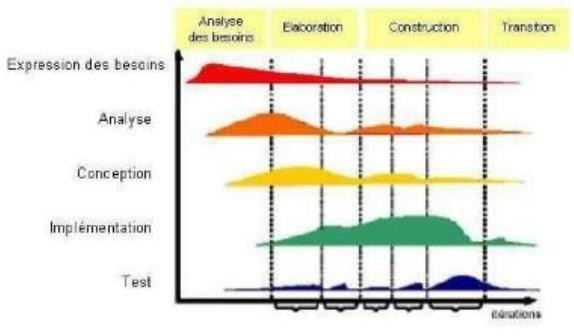
\includegraphics[width=0.8\linewidth]{image30.png}
	\caption{Activit\'{e} et phases d'UP}
	
\end{figure}

\chapter{Outils et matériel}


\noindent \begin{flushleft}
	
	
	\noindent 
	
	\noindent 
	
	\noindent 
	
	\section{Internet des objets (IoT)}
	
	\noindent 
	
	\noindent L'Internet des objets (IoT) est une nouvelle technologie qui se base sur des dispositifs informatiques interd\'{e}pendants, dot\'{e}s d'identifiants uniques (UID) et de la possibilit\'{e} de transf\'{e}rer des donn\'{e}es sur un r\'{e}seau sans n\'{e}cessiter l'interaction humaine.
	
	\noindent 
	
	\noindent 574727413La d\'{e}finition de l'Internet des objets a \'{e}volu\'{e} en raison de la convergence de plusieurs technologies, de l'analyse en temps r\'{e}el, de l'apprentissage automatique, des capteurs de produits et des syst\`{e}mes int\'{e}gr\'{e}s. [1] Les domaines traditionnels des syst\`{e}mes embarqu\'{e}s, des r\'{e}seaux de capteurs sans fil, des syst\`{e}mes de contr\^{o}le, de l'automatisation (y compris l'automatisation de la maison et du b\^{a}timent) et d'autres contribuent tous \`{a} permettre l'Internet des objets. 574727413UWUtilisateur Windows5747274131736735498https://accueil.edcloud.fr/snt-n1-5/
	
	\noindent 
	
	\noindent 
		\begin{figure}[H]
		\centering
		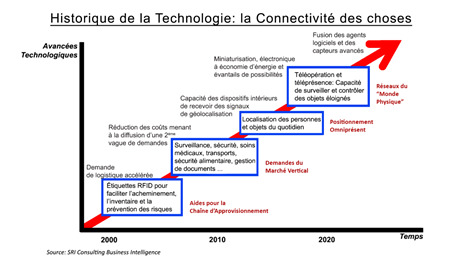
\includegraphics[width=0.8\linewidth]{image31}
		\caption{Historique de l'IoT.}
		
	\end{figure}

	
	\noindent 
	
	\noindent L'internet est d\'{e}fini comme~:
	
	\noindent 
	
	\noindent « R\'{e}unir des personnes, des processus, des donn\'{e}es et des \'{e}l\'{e}ments pour \'{e}tablir des connexions en r\'{e}seau plus pertinente et plus utile que jamais, en transformant les informations en actions qui cr\'{e}er de nouvelles capacit\'{e}s, des exp\'{e}riences plus riches et des opportunit\'{e}s \'{e}conomiques sans pr\'{e}c\'{e}dent pour les entreprises, les particuliers et les pays. » [IoT 15]. Par CISCO
	
	\noindent 
	
	\noindent 
	
	\noindent 
	
	\noindent Comme indiqu\'{e} dans la d\'{e}finition des IoT, Un objet dans l'Internet des objets a deux caract\'{e}ristiques : 
	
	\noindent $\mathrm{\checkmark}$ Un identifiant unique~: une adresse IP dans un r\'{e}seau. 
	
	\noindent $\mathrm{\checkmark}$ Il doit \^{e}tre capable de transf\'{e}rer des donn\'{e}es sur le r\'{e}seau pour communiquer avec son environnement
	
	\noindent 
	
	\noindent 
	
	\noindent 
	
	
	
	\noindent 
	
	\noindent Plusieurs \'{e}v\`{e}nements qui pr\'{e}c\`{e}dent l'internet des objets ont acc\'{e}l\'{e}rer son apparition, la figure X ci-dessous montre l'\'{e}volution d'internet 
	
	\noindent 
	
	\begin{figure}[H]
		\centering
		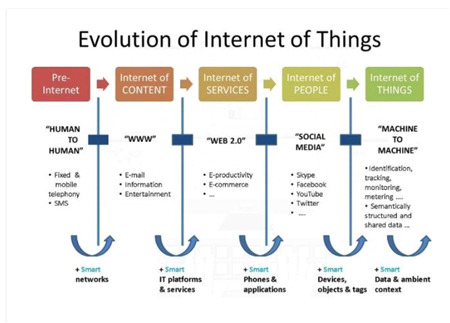
\includegraphics[width=0.8\linewidth]{image32}
		\caption{Evolution de l'internet.}

	\end{figure}
	
	
	\noindent 
	
	\noindent 1- la phase pr\'{e}-internet, la communication «~Humain \`{a} Humain~» qui se base sur la t\'{e}l\'{e}phonie fixe et mobile et les services de messageries SMS
	
	\noindent 2- la phase Internet du contenu, l'apparition du r\'{e}seau internet et les m\'{e}thodes d'acc\`{e}s associ\'{e}es d\'{e}nomm\'{e}s World Wide Web «~WWW~», qui a engendr\'{e} les courriers \'{e}lectronique «~Emails~» et les sites informatiques 
	
	\noindent 
	
	\noindent 3- la phase internet du service , L'\'{e}volution des r\'{e}seaux Internet a cr\'{e}\'{e} des plates-formes et des services informatiques qui ont naissance au WEB 2.0 avec les diff\'{e}rentes plateformes de commerce \'{e}lectronique et de productivit\'{e} \'{e}lectronique qui nous permettent par exemple de faire des achats en ligne.
	
	\noindent 
	
	\noindent 4- la phase internet des gens, l'invention des smartphones et le nombre \'{e}normes de l'application qui l'a suivi «~Facebook, twitter, Skype ...etc.~»
	
	\noindent 
	
	\noindent 5- Enfin, l'augmentation et la diversit\'{e} des technologies mobiles et embarqu\'{e}es. L'interaction machine \`{a} machine est devenue possible, une nouvelle g\'{e}n\'{e}ration de l'utilisation d'Internet \'{e}tait n\'{e}e : l'Internet des objets. 
	
	\noindent 
	
	\subsection{Types d'objet connect\'{e}s }
	
	\noindent 
	
	En mars 2015, le comit\'{e} Internet Architecture Board (IAB) 9 \'{e}dite la RFC10 7452. Il propose quatre mod\`{e}les communs d'interactions entre des acteurs de l'IdO11 [voir ROX 2017, p. 64] :
	
	\noindent 
\end{flushleft}

\begin{enumerate}
	\item  \textbf{\textit{La communication entre objets}}, ce mod\`{e}le est bas\'{e} sur une communication sans-fil entre deux objets Les informations sont transmises gr\^{a}ce \`{a} l'int\'{e}gration d'une technologie de communication sans fil comme le Bluetooth Low Energy (BLE), wifi ad-hoc sans la n\'{e}cessit\'{e} d'\^{e}tre connect\'{e}s \`{a} internet
\end{enumerate}

\noindent \begin{flushleft}
	
\end{flushleft}

\begin{enumerate}
	\item  La communication des objets vers une passerelle~: ce mod\`{e}le est bas\'{e} sur un interm\'{e}diaire «~Passerelle~» qui fait le lien entre les capteurs et l'objet communicant~(Smartphone par exemple)
\end{enumerate}

\noindent \begin{flushleft}
	
\end{flushleft}

\begin{enumerate}
	\item  La communication par r\'{e}seau IoT~: Les objets connect\'{e}s dans ce type utilisent les protocoles M2M (machine to machine) et sont directement connect\'{e}s \`{a} internet gr\^{a}ce \`{a} une technologie embarqu\'{e}e dans l'objet en question.
\end{enumerate}

\noindent \begin{flushleft}
	
	
	\noindent 
	
	\noindent 
	
	\noindent 
	
	\noindent 
	
	\noindent 
	
	\noindent 
	
	\noindent 
	
	\subsection{Domaines d'application de l'IoT :}
	\noindent 
\end{flushleft}

\noindent 
\paragraph{LA MAISON}

\noindent \begin{flushleft}
	La maison connect\'{e}e dispose de syst\`{e}mes automatiques tr\`{e}s avanc\'{e}s comme le contr\^{o}le de l'\'{e}clairage, de la s\'{e}curit\'{e}, de la fermeture ou de l'ouverture d'issues (portes+ fen\^{e}tres) ainsi que d'autres fonctions.~ Elle est aussi capable de participer \`{a} de nombreux aspects de la vie quotidienne comme le r\'{e}frig\'{e}rateur de Samsung,~Family Hub, qui peut effectuer l'inventaire de son stock~; proposer des menus ou commander du r\'{e}approvisionnement.
	
	\noindent ~
\end{flushleft}

\noindent 
\paragraph{LE SPORT}

\noindent \begin{flushleft}
	Des capteurs en tout genre ont fait leur apparition dans le monde du sport, qui est un des domaines privil\'{e}gi\'{e}s dans le secteur des objets connect\'{e}s. Le smartphone peut maintenant, gr\^{a}ce \`{a} de nombreuses applications, aider les personnes \`{a} contr\^{o}ler leur activit\'{e} sportive, leurs progr\`{e}s, leur alimentation et bien d'autre. Nous pouvons voir parmi les objets connect\'{e}s les fixations de snowboard~Cerevo~qui permettent de mesurer les performances et de les combiner \`{a} une vid\'{e}o qui est film\'{e}e gr\^{a}ce \`{a} une cam\'{e}ra int\'{e}gr\'{e}e. Nous retrouvons aussi~Xensr~qui est un capteur pour le sport de glisse r\'{e}coltant une multitude d'informations sur la vitesse des longueurs de sauts et le temps pass\'{e} en l'air.
	
	\noindent ~
\end{flushleft}

\noindent 
\paragraph{LE LOISIR}

\noindent \begin{flushleft}
	Les loisirs profitent aussi des objets connect\'{e}s et deviennent des loisirs connect\'{e}s qui nous facilitent la vie~; nous pouvons y retrouver les drones connect\'{e}s~; les jouets connect\'{e}s~ainsi que les voyage connect\'{e}s qui facilitent les d\'{e}parts en vacances et s\'{e}curisent le transport gr\^{a}ce \`{a} des valises de haute s\'{e}curit\'{e} comme la~Blue Smart~qui permet aux voyageurs de pouvoir retrouver leur valise \`{a} l'aide de leur t\'{e}l\'{e}phone portable mais aussi de pouvoir contr\^{o}ler son poids et de la verrouiller pour emp\^{e}cher les vols.
	
	\noindent ~
\end{flushleft}

\noindent 
\paragraph{LA SANT\'{E} ET LE BIEN-\^{E}TRE}

\noindent \begin{flushleft}
	La sant\'{e} connect\'{e}e est un ensemble de syst\`{e}me technologique visant \`{a} pr\'{e}server durablement la sant\'{e}. Le dispositif va enregistrer toutes les activit\'{e}s du corps afin d'en faire un compte rendu d\'{e}taill\'{e} sur le t\'{e}l\'{e}phone, la tablette ou l'ordinateur de son utilisateur.
	
	\noindent Contr\^{o}ler sa sant\'{e} devient alors un geste banal et rassurant, car les donn\'{e}es sont obtenues en temps r\'{e}el et peuvent \^{e}tre transmises imm\'{e}diatement au m\'{e}decin. La balance connect\'{e}e, notamment celle propos\'{e}e par~withings, permet de mesurer le poids et l'IMC. Elle peut \'{e}galement \^{e}tre utilis\'{e}e comme unit\'{e} de mesure de la masse grasse, maigre, musculaire, osseuse, hydrique, visc\'{e}rale et \^{e}tre en bonne indicatrice de la temp\'{e}rature ambiante et du pourcentage d'humidit\'{e}.
	
	\noindent ~
\end{flushleft}

\noindent 
\paragraph{LA MODE ET ACCESSOIRES}

\noindent \begin{flushleft}
	Les objets connect\'{e}s concernant la mode se d\'{e}veloppent, ainsi gr\^{a}ce \`{a} la gamme de bijoux~Altruis~ vous pourrez voir le plus important de vos notifications smartphone sous forme de vibrations.
	
	\noindent Les ceintures connect\'{e}es, elles, permettent de nous faire adopter une bonne posture tout enregistrant sur le t\'{e}l\'{e}phone les progr\`{e}s r\'{e}alis\'{e}s ou de contr\^{o}ler le tour de taille afin de pr\'{e}venir lors d'une prise ou d'une perte de poids.
	
	\noindent ~
\end{flushleft}

\noindent 
\paragraph{LE TRANSPORT}

\noindent \begin{flushleft}
	Les objets connect\'{e}s dans l'automobile vont combler les passionn\'{e}s cependant il faudra encore quelques ann\'{e}es avant de pouvoir d\'{e}velopper compl\'{e}tement ces technologies de mani\`{e}re efficaces. Quelques produits sont d\'{e}j\`{a} sur le march\'{e} comme le~casque de moto connect\'{e}~qui r\'{e}gularise toutes les difficult\'{e}s rencontr\'{e}es (recevoir des appels, vision total de l'entourage, envoyer des messages par voie orale). Nous connaissons aussi la voiture connect\'{e}es qui retranscrit le menu de votre portable sur son tableau de bord d\`{e}s que l'on y rentre.
	
	\noindent ~
\end{flushleft}

\noindent 
\paragraph{~LES MULTIM\'{E}DIA}

\noindent \begin{flushleft}
	Le multim\'{e}dia est un environnement propice au d\'{e}veloppement des objets connect\'{e}s et de toutes les technologies connect\'{e}es.
	
	\noindent La t\'{e}l\'{e}vision connect\'{e}e peut acc\'{e}der \`{a} internet et \`{a} de nombreux r\'{e}seaux sociaux et d'applications tels que YouTube, Dailymotion ou encore Facebook ou Twitter. Un bracelet connect\'{e},~KipstR, sera aussi bient\^{o}t commercialis\'{e}, il servira \`{a} rep\'{e}rer le moment o\`{u} une personne s'endort devant la t\'{e}l\'{e}vision et programme un enregistrement pour rattraper les choses manqu\'{e}es.
	
	\noindent ~
\end{flushleft}

\noindent 
\paragraph{~LES ANIMAUX}

\noindent \begin{flushleft}
	De nombreux objets connect\'{e}s existent pour rester en contact avec les animaux lors de d\'{e}placement, c'est notamment le but de la cam\'{e}ra en forme de cube,~Petcube, \'{e}quip\'{e}e d'un micro et d'un haut-parleur. Il existe aussi des jeux connect\'{e}s, \'{e}quip\'{e}s de trois touches tactiles afin d'occuper les animaux la journ\'{e}e.
	
	\noindent ~
\end{flushleft}

\noindent 
\paragraph{LES B\'{E}B\'{E}S}

\noindent \begin{flushleft}
	M\^{e}me les nouveaux n\'{e}s sont touch\'{e}s par la r\'{e}volution technologique, ainsi il existe des baby phones, comme~l'\'{e}coute b\'{e}b\'{e} de Philips,~connect\'{e}s au portable avec des alertes quand le b\'{e}b\'{e} pleure ou encore des p\`{e}se-b\'{e}b\'{e}s connect\'{e}s qui permettent de garder un {\oe}il sur sa courbe.
	
	\noindent 
	
	\noindent 
	
	\noindent 
	
	\noindent 
	
	\noindent 
	
	\noindent 
	
	\noindent 
	
	\noindent 
	
	\subsection{Architecture g\'{e}n\'{e}ral d'un system IoT}
	
	\noindent Pour concevoir un syst\`{e}me IoT, on doit s'int\'{e}resser principalement aux aspects suivants:
	
	\noindent \textbf{Collecte de donn\'{e}es }(collecte des donn\'{e}es \`{a} partir de p\'{e}riph\'{e}riques \'{e}lectroniques comme les capteurs, cam\'{e}ras, ...etc.).
\end{flushleft}

\begin{enumerate}
	\item \begin{enumerate}
		\item  Traitement des donn\'{e}es.
		
		\item  Analyses de donn\'{e}es.
		
		\item  Toute architecture IoT doit comporter les composants de base suivants :
	\end{enumerate}
\end{enumerate}

\noindent \begin{flushleft}
	\textbf{Instruments : }(Ceci est principalement li\'{e} \`{a} l'\'{e}lectronique) qui peuvent \^{e}tre branch\'{e}s sur un r\'{e}seau informatique avec une adresse IP particuli\`{e}re.
	
	\noindent \textbf{Infrastructure : }besoin d'un serveur et une connexion r\'{e}seau pour garder l'ensemble op\'{e}rationnel. Il est tr\`{e}s similaire aux LAN, WAN ou Internet, et doit avoir ses serveurs connect\'{e}s \`{a} Internet, ou li\'{e} \`{a} un environnement de service Cloud virtuel. Microsoft, IBM, Amazon et la plupart des grands acteurs fournissent des infrastructures pour IoT. Le choix d\'{e}pend du besoin particulier.
	
	\noindent \textbf{Codage : }cette partie concerne l'utilisation des langages de programmation pour r\'{e}aliser le logique m\'{e}tier associ\'{e} au syst\`{e}me IoT.
	
	\noindent \textbf{S\'{e}curit\'{e} : }Cela rev\^{e}t une importance capitale en ce qui concerne l'IoT. Lorsqu'\`{a} la Connection d'un plus grand nombre de p\'{e}riph\'{e}riques ensemble, cela ouvre beaucoup de vuln\'{e}rabilit\'{e}s. Il existe toujours une menace pour les donn\'{e}es personnelles, car cela pourrait \^{e}tre compromis si elles ne sont pas prises en charge correctement.
\end{flushleft}

\noindent \textbf{Gestion des donn\'{e}es : }Le traitement des quantit\'{e}s massives de donn\'{e}es dans l'IoT. Besoin d'un grand syst\`{e}me de donn\'{e}es comme Hadoop et Apache Storm pour \^{e}tre en place pour la gestion et le traitement des donn\'{e}es.

\noindent 
\begin{flushleft}
	\textbf{Analyse des donn\'{e}es : }Une fois que les donn\'{e}es sont trait\'{e}es et g\'{e}r\'{e}es, Il existe plusieurs \'{e}l\'{e}ments essentiels qui peuvent \^{e}tre d\'{e}chiffr\'{e}s des « donn\'{e}es inutilis\'{e}s ». L'intelligence des donn\'{e}es, l'exploration de donn\'{e}es, ...etc. sont quelques-unes des techniques que pouvait utiliser pour analyser les donn\'{e}es et obtenir des informations significatives qui conduiraient l'\'{e}cosyst\`{e}me IoT [8].
	
	\subsection{Les plateformes IoT:}
	La plateforme~IoT~rassemble un ensemble de services qui permettent de collecter, stocker, corr\'{e}ler, analyser et exploiter des donn\'{e}es. Elle fait ainsi r\'{e}f\'{e}rence au logiciel de support qui connecte l'ensemble du syst\`{e}me IoT, en facilitant la communication, le flux de donn\'{e}es, la gestion des p\'{e}riph\'{e}riques et la fonctionnalit\'{e} des applications. La plateforme connecte~les appareils \`{a} un cloud gr\^{a}ce \`{a} des options de connectivit\'{e} flexibles. 
	
	\noindent Pour les d\'{e}veloppeurs, une plateforme IoT fournit un ensemble de fonctionnalit\'{e}s pr\^{e}tes \`{a} l'emploi qui acc\'{e}l\`{e}re le d\'{e}veloppement d'applications pour les p\'{e}riph\'{e}riques connect\'{e}s, tout en prenant en charge l'\'{e}volutivit\'{e} et la compatibilit\'{e} entre p\'{e}riph\'{e}riques. Elle peut \'{e}galement servir de middleware lorsqu'elle connecte les p\'{e}riph\'{e}riques distants aux applications utilisateurs (ou autres p\'{e}riph\'{e}riques) tout en g\'{e}rant les interactions entre le mat\'{e}riel et les couches des applications574727417UWUtilisateur Windows5747274171736735644https://www.journaldunet.fr/web-tech/dictionnaire-de-l-iot/1440690-plateforme-iot-definition-comparatif-device-management/
	
	\noindent 
	
	\noindent 
	
	\noindent La plate-forme IoT garantit une int\'{e}gration transparente avec diff\'{e}rents mat\'{e}riels en utilisant une gamme de protocoles de communication populaires, en appliquant diff\'{e}rents types de topologie (connexion directe ou passerelle) et en utilisant des SDK (Software D\'{e}veloppent Kit) si n\'{e}cessaire.
	
	\noindent 
	
	\noindent Exemple~de plateformes IoT~: 
	
	\noindent $\mathrm{\checkmark}$ AWS IoT Platform. 
	
	\noindent $\mathrm{\checkmark}$ Blynk IoT Platform. 
	
	\noindent $\mathrm{\checkmark}$ EVRYTHNG - IoT Smart Products Platform. 
	
	\noindent $\mathrm{\checkmark}$ IBM IoT Foundation Device Cloud. 
	
	\noindent $\mathrm{\checkmark}$ ParStream - IoT Analytics Platform. 
	
	\noindent $\mathrm{\checkmark}$ Kaa IoT platform. 
	
	\noindent $\mathrm{\checkmark}$ Google IOT platform.
	
	\noindent  $\mathrm{\checkmark}$ Microsoft azure IoT platform.
	
	\noindent  $\mathrm{\checkmark}$ CarrIoTs IoT platform.
	
	\noindent 
	
	\noindent 
	
	\noindent 
	
	\noindent 
	
	\noindent 
	
	\noindent 
	
	\noindent 
	
	\section{Les syst\`{e}mes embarqu\'{e}s}
	
	\paragraph{D\'{e}finition 1:}
	
	\noindent 574727418Un~\textbf{syst\`{e}me embarqu\'{e}}~est un syst\`{e}me complexe qui int\`{e}gre du logiciel et du mat\'{e}riel con\c{c}us ensemble afin de fournir des fonctionnalit\'{e}s donn\'{e}es. Il contient g\'{e}n\'{e}ralement un ou plusieurs~\textbf{microprocesseurs}~destin\'{e}s \`{a} ex\'{e}cuter un ensemble de~\textbf{programmes}~d\'{e}finis lors de la conception et stock\'{e}s dans des~\textbf{m\'{e}moires}. Le~\textbf{syst\`{e}me mat\'{e}riel}~et l'\textbf{application~}(\textbf{logiciel}) sont intimement li\'{e}s et immerg\'{e}s dans le mat\'{e}riel et ne sont pas aussi facilement discernables comme dans un~\textbf{environnement de travail}~classique de type ordinateur de bureau PC (Personale Computer).
	
	\paragraph{D\'{e}finition 2:}
	
	\noindent 574727419Les syst\`{e}mes embarqu\'{e}s sont des syst\`{e}mes informatiques mais peuvent ne pas comporter d'interface utilisateur par exemple, sur des p\'{e}riph\'{e}riques dans lesquels le syst\`{e}me int\'{e}gr\'{e} est con\c{c}u pour effectuer une t\^{a}che unique vers une interface utilisateur graphique complexe, telle que dans les appareils mobiles. L'interface utilisateur peut faire r\'{e}f\'{e}rence \`{a} des boutons, des voyants, des capteurs tactiles, etc574727419UWUtilisateur Windows5747274191736735659Margaret Rouse. embedded system.. 
	
	\noindent 
	
	\subsection{Caract\'{e}ristiques}
	
	\noindent 574727420Les caract\'{e}ristiques principales d'un syst\`{e}me \'{e}lectronique embarqu\'{e} sont~:
\end{flushleft}

\begin{enumerate}
	\item  L'autonomie~: D\'{e}di\'{e}e \`{a} une application sp\'{e}cifique.
	
	\item  Ex\'{e}cution temps r\'{e}el~: l'importance majeure des temps de r\'{e}ponses 
	
	\item  $\mathrm{\centerdot}$ Fiabilit\'{e} et s\'{e}curit\'{e} de fonctionnement
\end{enumerate}

\begin{flushleft}
	$\mathrm{\centerdot}$ Consommation d'\'{e}nergie maitris\'{e}e574727420UWUtilisateur Windows5747274201736735667Etienne Messerli
	
	\noindent Cours~Les systemes embarqu\'{e}s
\end{flushleft}

\noindent \begin{enumerate}
	\item Haute ecole d'ing\'{e}nerie et de gestion du canton de vaud
\end{enumerate}

\noindent \begin{flushleft}
	
	
	\noindent 
	
	\noindent 
	
	\noindent 
	
	\noindent 
	
	\noindent 
	
	\noindent 
	
	\noindent 
	
	\noindent 
	
	\noindent 
	
	\noindent 
	
	\subsection{Syst\`{e}mes informatiques et Syst\`{e}mes 574727421embarqu\'{e}s}
	

\end{flushleft}


\noindent \begin{flushleft}
	
	
	\noindent Les diff\'{e}rences entre les deux syst\`{e}mes se r\'{e}sument dans le tableau r\'{e}capitulatif ci-dessous
	
	\noindent 
\end{flushleft}

\begin{tabular}{|p{2.3in}|p{2.3in}|} \hline 
	\textbf{Syst\`{e}me Informatique} & \textbf{Syst\`{e}me Embarqu\'{e}} \\ \hline 
	Processeur standard\newline  Multiples unit\'{e}s fonctionnelles (flottant)\newline  Vitesse \'{e}lev\'{e}e ($\mathrm{>}$ GHz)\newline  Consommation \'{e}lectrique \'{e}lev\'{e}e\newline  Chaleur\newline  Taille\newline MMU (m\'{e}moire virtuelle) OS\newline Cache\newline Grand nombre de p\'{e}riph\'{e}riques & Processeur d\'{e}di\'{e} (contr\^{o}leur)\newline  Architecture adapt\'{e}e\newline  Vitesse faible ($\mathrm{\sim}$200 MHz)\newline  8-32bits: m\'{e}moire limit\'{e}e\newline  Basse consumation\newline  Petite taille, grand volume =$\mathrm{>}$ faible co\^{u}t Processeur DSP (traitements)\newline  Tr\`{e}s puissants Quelques Mo de m\'{e}moire RTOS \\ \hline 
\end{tabular}

\begin{flushleft}
	
	
	\noindent 
	
	\subsection{Classification des syst\`{e}mes embarqu\'{e}s}
	

\end{flushleft}


\noindent \begin{flushleft}
	Les syst\`{e}mes embarqu\'{e}s sont classifi\'{e}s en trois syst\`{e}mes :
	
	\noindent \textit{Syst\`{e}me Transformationnel}
	
	\noindent Qui lit ses donn\'{e}es et ses entr\'{e}es lors de son d\'{e}marrage, qui fournit ses sorties, puis meurt 
	
	\noindent \textit{Syst\`{e}me Interactif}
	
	\noindent Syst\`{e}me en interaction quasi permanente avec son environnement, y compris apr\`{e}s l'initialisation du syst\`{e}me ; la r\'{e}action du syst\`{e}me est d\'{e}termin\'{e}e par les \'{e}v\'{e}nements re\c{c}us et par l'\'{e}tat courant (fonction des \'{e}v\'{e}nements et des r\'{e}actions pass\'{e}s), le rythme de l'interaction est d\'{e}termin\'{e} par le syst\`{e}me et non par l'environnement 
	
	\noindent \textit{Syst\`{e}me R\'{e}actif ou Temps R\'{e}el}
	
	\noindent Syst\`{e}me en interaction permanente avec son environnement, y compris apr\`{e}s l'initialisation du syst\`{e}me ; la r\'{e}action du syst\`{e}me est d\'{e}termin\'{e}e par les \'{e}v\'{e}nements re\c{c}us et par l'\'{e}tat courant (fonction des \'{e}v\'{e}nements et des r\'{e}actions pass\'{e}es), mais le rythme de l'interaction est d\'{e}termin\'{e} par l'environnement et non par le syst\`{e}me 
	
	\noindent 
	
	\noindent 
	
	\subsection{Domaines d'application des syst\`{e}mes embarqu\'{e}s}
\end{flushleft}

\noindent \begin{flushleft}
	
	
	\noindent \textbf{Domaine grand public }
	
	$\mathrm{\centerdot}$ Smart phone, console de jeux, appareil photos, lecteur audio, ...  
	
	\noindent \textbf{Moyens de transport }
	
	\noindent $\mathrm{\centerdot}$ Gestion moteur/entrainement, ordinateur de bord, ABS, GPS, syst\`{e}me navigation, syst\`{e}me d'aide (EPS, ..), =$\mathrm{>}$ automobiles, avions, trains, bateau, v\'{e}hicule \'{e}lectrique, {\dots} 
	
	\noindent  \textbf{Equipement} m\'{e}dicaux (diagnostic, th\'{e}rapeutique, vital)
	
	\noindent  $\mathrm{\centerdot}$ Imagerie (rayon X, ultra-sons, IRM), endoscopie, cam\'{e}ra, monitoring, perfusion, lasers, chirurgie, stimulateur cardiaque, {\dots} 
	
	\noindent  \textbf{Equipements} de t\'{e}l\'{e}communication $\mathrm{\centerdot}$ 
	
	Mobile, routeur, Gateway, satellite, {\dots} 
	
	\noindent   \textbf{Equipement} industriels
	
	\noindent  $\mathrm{\centerdot}$ commande, contr\^{o}le r\'{e}partit, capteurs intelligents, ...
	
	\noindent  
	
	\noindent 
	
	\noindent 
	
	\section{Raspberry }
\end{flushleft}

\noindent Le Raspberry Pi est un ordinateur de la taille d'une carte de cr\'{e}dit et pouvant \^{e}tre connect\'{e} \`{a} un ordinateur. Moniteur ou t\'{e}l\'{e}viseur et utilise un clavier et une souris standard. Il est capable de faire tout ce qu'on attend d'un ordinateur de bureau \`{a} faire, de naviguer sur Internet et de lire des vid\'{e}os haute d\'{e}finition, \'{e}diter des feuilles de calcul, du traitement de texte et jouer \`{a} des jeux. [Rasb].

\noindent De plus, le Raspberry Pi a la capacit\'{e} d'interagir avec le monde ext\'{e}rieur et a \'{e}t\'{e} utilis\'{e} dans un large \'{e}ventail de projets de fabrication num\'{e}rique, allant des appareils de musique aux d\'{e}tecteurs des stations m\'{e}t\'{e}o.

\noindent \begin{flushleft}
	
	
		\begin{figure}[H]
		\centering
		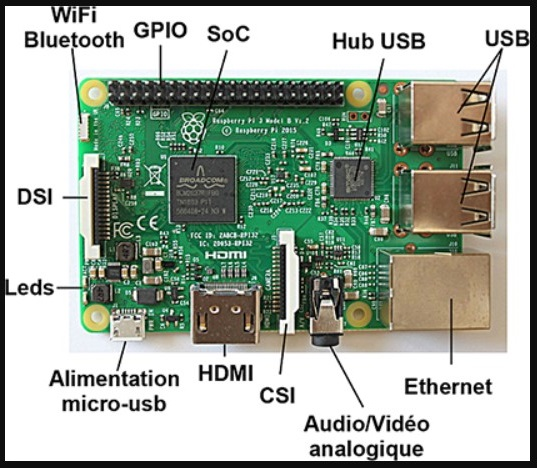
\includegraphics[width=0.8\linewidth]{image33}
		\caption{Évolution de l'internet.}
		
		\end{figure}
	
\end{flushleft}

\subsection{Composants d'une carte Raspberry}

\noindent \textbf{Processeur / GPU ARM }: Il s'agit d'un syst\`{e}me Broadcom BCM2835 sur puce (SoC) compos\'{e} d'une unit\'{e} centrale de traitement ARM (CPU) et d'un graphique Videocore 4 unit\'{e} de traitement (GPU). La CPU g\`{e}re tous les calculs qui font un travail sur ordinateur (prendre des entr\'{e}es, faire des calculs et produire des sorties), et le GPU g\`{e}re la sortie graphique.

\noindent \begin{flushleft}
	
\end{flushleft}

\noindent \textbf{GPIO }: Ce sont des points de connexion d'entr\'{e}e / sortie \`{a} usage g\'{e}n\'{e}ral qui permettent de connecter d'autres hardware.

\noindent \begin{flushleft}
	
\end{flushleft}

\noindent \textbf{RCA }: Une prise RCA permet la connexion de t\'{e}l\'{e}viseurs analogiques et d'autres p\'{e}riph\'{e}riques de sortie similaires.

\noindent \begin{flushleft}
	
\end{flushleft}

\noindent \textbf{Sortie audio }: C'est une prise standard de 3,55 millim\`{e}tres pour la connexion de la sortie audio des appareils tels que des \'{e}couteurs ou des haut-parleurs. Il n'y a pas d'audio dans.

\noindent \begin{flushleft}
	
\end{flushleft}

\noindent \textbf{LED Diodes }: \'{e}lectroluminescentes, pour tous les besoins en indicateur lumineux.

\noindent \begin{flushleft}
	
\end{flushleft}

\noindent \textbf{USB }: C'est un port de connexion commun pour les p\'{e}riph\'{e}riques de tous types (y compris la souris et le clavier). Le mod\`{e}le A en a un et le mod\`{e}le B en compte deux. Un concentrateur USB peut \^{e}tre utilis\'{e} pour augmenter le nombre de ports USB.

\noindent \begin{flushleft}
	
\end{flushleft}

\noindent \textbf{HDMI }: Permet de brancher un t\'{e}l\'{e}viseur haut d\'{e}finition ou tout autre appareil compatible utilisant un c\^{a}ble HDMI.

\noindent \begin{flushleft}
	
\end{flushleft}

\noindent \textbf{Source de courant : }Il s'agit d'un connecteur d'alimentation micro USB 5v dans lequel vous pouvez brancher votre appareil compatible.

\noindent \begin{flushleft}
	
\end{flushleft}

\noindent \textbf{Lecteur de carte SD (DSI) }: Il s'agit d'un compartiment pour carte SD de taille normale. Une carte SD avec un syst\`{e}me d'exploitation (OS) install\'{e} est requise pour l'amor\c{c}age du p\'{e}riph\'{e}rique. Le syst\`{e}me d'exploitation requis est disponible en achat, et t\'{e}l\'{e}chargeable \'{e}galement avec une machine Linux.

\noindent \begin{flushleft}
	
\end{flushleft}

\noindent \textbf{Ethernet }: Permet un acc\`{e}s au r\'{e}seau filaire et n'est disponible que sur le Mod\`{e}le B.


\section{Plateformes et langages :}
\subsection{PhpStorm}
PhpStorm est un éditeur pour les langages HTML, CSS, PHP et Javascript PhpStorm est un éditeur pour PHP3, HTML, CSS et JavaScript4, édité par JetBrains.
Une interface utilisateur pour les logiciels de tests tels que PHPUnit ; Le débogage pas-à-pas et le profilage de code en dialoguant avec Xdebug.
Il permet aussi de visualiser l'architecture de bases de données de différentes sources (MySQL, SQLite, etc.).
Enfin, il permet l'intégration d'outils d'opérations serveur comme Vagrant, Docker, une console SSH et bien d'autres outils.
PHPStorm est écrit en Java, et ses utilisateurs peuvent lui adjoindre des extensions fournies par JetBrains, une tierce partie ou écrites par eux-mêmes.
Toutes sortes d'outils destinés à facilité et accélérer le travail du développeur : aides à l'apprentissage des touches de raccourci, manipulation de texte, coloration de parenthèses, etc.
Enfin, il est possible d'utiliser gratuitement PHPStorm via le Early Access Program10, qui permet d'évaluer la prochaine version majeure du logiciel.
	\begin{figure}[H]
	\centering
	\includegraphics[width=0.3\linewidth]{phpstorm}
	\caption{Logo PhpStorm.}
	
\end{figure}
\subsection{Android Studio}
Android Studio est un environnement de développement pour développer des applications mobiles Android. Il est basé sur IntelliJ IDEA et utilise le moteur de production Gradle. Il peut être téléchargé sous les systèmes d'exploitation Windows, macOS, Chrome OS et Linux4.
	\begin{figure}[H]
	\centering
	\includegraphics[width=0.3\linewidth]{android}
	\caption{Logo Android Studion.}
	
\end{figure}

\subsection{PHP}
HP: Hypertext Preprocessor5, plus connu sous son sigle PHP (sigle auto-référentiel), est un langage de programmation libre6, principalement utilisé pour produire des pages Web dynamiques via un serveur HTTP5, mais pouvant également fonctionner comme n'importe quel langage interprété de façon locale. PHP est un langage impératif orienté objet.
PHP a permis de créer un grand nombre de sites web célèbres, comme Facebook, Wikipédia, etc.7 Il est considéré comme une des bases de la création de sites web dits dynamiques mais également des applications web.
\begin{figure}[H]
	\centering
	
\includegraphics[width=0.3\linewidth]{php}
	\caption{Logo PHP.}
	
\end{figure}

\subsection{Javascript}
JavaScript est un langage de programmation de scripts principalement employé dans les pages web interactives mais aussi pour les serveurs2 avec l'utilisation (par exemple) de Node.js3. C'est un langage orienté objet à prototype, c'est-à-dire que les bases du langage et ses principales interfaces sont fournies par des objets qui ne sont pas des instances de classes, mais qui sont chacun équipés de constructeurs permettant de créer leurs propriétés, et notamment une propriété de prototypage qui permet d'en créer des objets héritiers personnalisés. En outre, les fonctions sont des objets de première classe. Le langage supporte le paradigme objet, impératif et fonctionnel. JavaScript est le langage possédant le plus large écosystème grâce à son gestionnaire de dépendances npm, avec environ 500 000 paquets en août 20174.
\begin{figure}[H]
	\centering
	
\includegraphics[width=0.3\linewidth]{js}
	\caption{Logo JavaScript.}
	
\end{figure}





\subsection{HTML}
Le HyperText Markup Language, généralement abrégé HTML ou dans sa dernière version HTML5, est le langage de balisage conçu pour représenter les pages web. C’est un langage permettant d’écrire de l’hypertexte, d’où son nom. HTML permet également de structurer sémantiquement et logiquement et de mettre en forme le contenu des pages, d’inclure des ressources multimédias dont des images, des formulaires de saisie et des programmes informatiques. Il permet de créer des documents interopérables avec des équipements très variés de manière conforme aux exigences de l’accessibilité du web. Il est souvent utilisé conjointement avec le langage de programmation JavaScript et des feuilles de style en cascade (CSS). HTML est inspiré du Standard Generalized Markup Language (SGML). Il s'agit d'un format ouvert.
\begin{figure}[H]
	\centering
	
\includegraphics[width=0.3\linewidth]{html}
	\caption{Logo HTML.}
	
\end{figure}

\subsection{JAVA}
Java est un langage de programmation orienté objet créé par James Gosling et Patrick Naughton, employés de Sun Microsystems, avec le soutien de Bill Joy (cofondateur de Sun Microsystems en 1982), présenté officiellement le 23 mai 1995 au SunWorld.
La société Sun a été ensuite rachetée en 2009 par la société Oracle qui détient et maintient désormais Java.
Une particularité de Java est que les logiciels écrits dans ce langage sont compilés vers une représentation binaire intermédiaire qui peut être exécutée dans une machine virtuelle Java (JVM) en faisant abstraction du système d'exploitation.
\begin{figure}[H]
	\centering
	
\includegraphics[width=0.3\linewidth]{java}
	\caption{Logo JAVA.}
	
\end{figure}

\subsection{XML}
L'Extensible Markup Language, généralement appelé XMLnote 1, « langage de balisage extensible1 » en français, est un métalangage informatique de balisage générique qui est un sous-ensemble du Standard Generalized Markup Language (SGML). Sa syntaxe est dite « extensible » car elle permet de définir différents langages avec pour chacun son vocabulaire et sa grammaire, comme XHTML, XSLT, RSS, SVG… Elle est reconnaissable par son usage des chevrons (<, >) encadrant les noms des balises. L'objectif initial de XML est de faciliter l'échange automatisé de contenus complexes (arbres, texte enrichi, etc.) entre systèmes d'informations hétérogènes (interopérabilité). Avec ses outils et langages associés, une application XML respecte généralement certains principes :


\subsection{CSS}
Les feuilles de style en cascade1, généralement appelées CSS de l'anglais Cascading Style Sheets, forment un langage informatique qui décrit la présentation des documents HTML et XML. Les standards définissant CSS sont publiés par le World Wide Web Consortium (W3C). Introduit au milieu des années 1990, CSS devient couramment utilisé dans la conception de sites web et bien pris en charge par les navigateurs web dans les années 2000.
\begin{figure}[H]
	\centering
	
\includegraphics[width=0.3\linewidth]{css}
	\caption{Logo CSS.}
	
\end{figure}

\subsection{XAMPP}
XAMPP est un ensemble de logiciels permettant de mettre en place un serveur Web local, un serveur FTP et un serveur de messagerie électronique. Il s'agit d'une distribution de logiciels libres (X (cross) Apache MariaDB Perl PHP) offrant une bonne souplesse d'utilisation, réputée pour son installation simple et rapide. Ainsi, il est à la portée d'un grand nombre de personnes puisqu'il ne requiert pas de connaissances particulières et fonctionne, de plus, sur les systèmes d'exploitation les plus répandus.
\begin{figure}[H]
	\centering
	
\includegraphics[width=0.3\linewidth]{xampp}
	\caption{Logo XAMPP.}
	
\end{figure}

\newpage
\bibliography{references} 
\bibliographystyle{ieeetr}

\end{document}